%%  A simple AAU report template.
%  2015-05-08 v. 1.2.0
%  Copyright 2010-2015 by Jesper Kjær Nielsen <jkn@es.aau.dk>
%
%  This is free software: you can redistribute it and/or modify
%  it under the terms of the GNU General Public License as published by
%  the Free Software Foundation, either version 3 of the License, or
%  (at your option) any later version.
%
%  This is distributed in the hope that it will be useful,
%  but WITHOUT ANY WARRANTY; without even the implied warranty of
%  MERCHANTABILITY or FITNESS FOR A PARTICULAR PURPOSE.  See the
%  GNU General Public License for more details.
%
%  You can find the GNU General Public License at <http://www.gnu.org/licenses/>.
%

%  A simple AAU report template.
%  2015-05-08 v. 1.2.0
%  Copyright 2010-2015 by Jesper Kjær Nielsen <jkn@es.aau.dk>
%
%  This is free software: you can redistribute it and/or modify
%  it under the terms of the GNU General Public License as published by
%  the Free Software Foundation, either version 3 of the License, or
%  (at your option) any later version.
%
%  This is distributed in the hope that it will be useful,
%  but WITHOUT ANY WARRANTY; without even the implied warranty of
%  MERCHANTABILITY or FITNESS FOR A PARTICULAR PURPOSE.  See the
%  GNU General Public License for more details.
%
%  You can find the GNU General Public License at <http://www.gnu.org/licenses/>.
%
\documentclass[11pt,twoside,a4paper,openright]{report}
%%%%%%%%%%%%%%%%%%%%%%%%%%%%%%%%%%%%%%%%%%%%%%%%
% Language, Encoding and Fonts
% http://en.wikibooks.org/wiki/LaTeX/Internationalization
%%%%%%%%%%%%%%%%%%%%%%%%%%%%%%%%%%%%%%%%%%%%%%%%
% Select encoding of your inputs. Depends on
% your operating system and its default input
% encoding. Typically, you should use
%   Linux  : utf8 (most modern Linux distributions)
%            latin1 
%   Windows: ansinew
%            latin1 (works in most cases)
%   Mac    : applemac
% Notice that you can manually change the input
% encoding of your files by selecting "save as"
% an select the desired input encoding. 
\usepackage[utf8]{inputenc}
% Make latex understand and use the typographic
% rules of the language used in the document.
\usepackage[danish,english]{babel}
% Use the palatino font
\usepackage[sc]{mathpazo}
\linespread{1.05}         % Palatino needs more leading (space between lines)
% Choose the font encoding
\usepackage[T1]{fontenc}
%%%%%%%%%%%%%%%%%%%%%%%%%%%%%%%%%%%%%%%%%%%%%%%%
% Graphics and Tables
% http://en.wikibooks.org/wiki/LaTeX/Importing_Graphics
% http://en.wikibooks.org/wiki/LaTeX/Tables
% http://en.wikibooks.org/wiki/LaTeX/Colors
%%%%%%%%%%%%%%%%%%%%%%%%%%%%%%%%%%%%%%%%%%%%%%%%
% load a colour package
\usepackage{xcolor}
\definecolor{aaublue}{RGB}{33,26,82}% dark blue
% The standard graphics inclusion package
\usepackage{graphicx}
% Set up how figure and table captions are displayed
\usepackage{caption}
\captionsetup{%
  font=footnotesize,% set font size to footnotesize
  labelfont=bf % bold label (e.g., Figure 3.2) font
}
% Make the standard latex tables look so much better
\usepackage{array,booktabs}
% Enable the use of frames around, e.g., theorems
% The framed package is used in the example environment
\usepackage{framed}

%%%%%%%%%%%%%%%%%%%%%%%%%%%%%%%%%%%%%%%%%%%%%%%%
% Mathematics
% http://en.wikibooks.org/wiki/LaTeX/Mathematics
%%%%%%%%%%%%%%%%%%%%%%%%%%%%%%%%%%%%%%%%%%%%%%%%
% Defines new environments such as equation,
% align and split 
\usepackage{amsmath}
% Adds new math symbols
\usepackage{amssymb}
% Use theorems in your document
% The ntheorem package is also used for the example environment
% When using thmmarks, amsmath must be an option as well. Otherwise \eqref doesn't work anymore.
\usepackage[framed,amsmath,thmmarks]{ntheorem}

%%%%%%%%%%%%%%%%%%%%%%%%%%%%%%%%%%%%%%%%%%%%%%%%
% Page Layout
% http://en.wikibooks.org/wiki/LaTeX/Page_Layout
%%%%%%%%%%%%%%%%%%%%%%%%%%%%%%%%%%%%%%%%%%%%%%%%
% Change margins, papersize, etc of the document
\usepackage[
  inner=28mm,% left margin on an odd page
  outer=41mm,% right margin on an odd page
  ]{geometry}
% Modify how \chapter, \section, etc. look
% The titlesec package is very configureable
\usepackage{titlesec}
\titleformat{\chapter}[display]{\normalfont\huge\bfseries}{\chaptertitlename\ \thechapter}{20pt}{\Huge}
\titleformat*{\section}{\normalfont\Large\bfseries}
\titleformat*{\subsection}{\normalfont\large\bfseries}
\titleformat*{\subsubsection}{\normalfont\normalsize\bfseries}
%\titleformat*{\paragraph}{\normalfont\normalsize\bfseries}
%\titleformat*{\subparagraph}{\normalfont\normalsize\bfseries}

% Clear empty pages between chapters
\let\origdoublepage\cleardoublepage
\newcommand{\clearemptydoublepage}{%
  \clearpage
  {\pagestyle{empty}\origdoublepage}%
}
\let\cleardoublepage\clearemptydoublepage

% Change the headers and footers
\usepackage{fancyhdr}
\pagestyle{fancy}
\fancyhf{} %delete everything
\renewcommand{\headrulewidth}{0pt} %remove the horizontal line in the header
\fancyhead[RE]{\small\nouppercase\leftmark} %even page - chapter title
\fancyhead[LO]{\small\nouppercase\rightmark} %uneven page - section title
\fancyhead[LE,RO]{\thepage} %page number on all pages
% Do not stretch the content of a page. Instead,
% insert white space at the bottom of the page
\raggedbottom
% Enable arithmetics with length. Useful when
% typesetting the layout.
\usepackage{calc}

%%%%%%%%%%%%%%%%%%%%%%%%%%%%%%%%%%%%%%%%%%%%%%%%
% Bibliography
% http://en.wikibooks.org/wiki/LaTeX/Bibliography_Management
%%%%%%%%%%%%%%%%%%%%%%%%%%%%%%%%%%%%%%%%%%%%%%%%
\usepackage[backend=bibtex,
  bibencoding=utf8
  ]{biblatex}
\addbibresource{bib/mybib}

%%%%%%%%%%%%%%%%%%%%%%%%%%%%%%%%%%%%%%%%%%%%%%%%
% Misc
%%%%%%%%%%%%%%%%%%%%%%%%%%%%%%%%%%%%%%%%%%%%%%%%
% Add bibliography and index to the table of
% contents
\usepackage[nottoc]{tocbibind}
% Add the command \pageref{LastPage} which refers to the
% page number of the last page
\usepackage{lastpage}
% Add todo notes in the margin of the document
\usepackage[
%  disable, %turn off todonotes
  colorinlistoftodos, %enable a coloured square in the list of todos
  textwidth=\marginparwidth, %set the width of the todonotes
  textsize=scriptsize, %size of the text in the todonotes
  ]{todonotes}

%%%%%%%%%%%%%%%%%%%%%%%%%%%%%%%%%%%%%%%%%%%%%%%%
% Hyperlinks
% http://en.wikibooks.org/wiki/LaTeX/Hyperlinks
%%%%%%%%%%%%%%%%%%%%%%%%%%%%%%%%%%%%%%%%%%%%%%%%
% Enable hyperlinks and insert info into the pdf
% file. Hypperref should be loaded as one of the 
% last packages
\usepackage[hidelinks]{hyperref}
\hypersetup{%
	pdfpagelabels=true,%
	plainpages=false,%
	pdfauthor={Author(s)},%
	pdftitle={Title},%
	pdfsubject={Subject},%
	bookmarksnumbered=true,%
	colorlinks=false,%
	citecolor=black,%
	filecolor=black,%
	linkcolor=black,% you should probably change this to black before printing
	urlcolor=black,%
	pdfstartview=FitH%
}


%%%%%%
% MY ADDITIOJNS:
%%%%%%

\setlength{\parindent}{0pt}

\usepackage{subcaption}% package inclusion and set up of the document
% see, e.g., http://en.wikibooks.org/wiki/LaTeX/Formatting#Hyphenation
% for more information on word hyphenation
\hyphenation{ex-am-ple hy-phen-a-tion short}
\hyphenation{long la-tex}
% 
%  A simple AAU report template.
%  2015-05-08 v. 1.2.0
%  Copyright 2010-2015 by Jesper Kjær Nielsen <jkn@es.aau.dk>
%
%  This is free software: you can redistribute it and/or modify
%  it under the terms of the GNU General Public License as published by
%  the Free Software Foundation, either version 3 of the License, or
%  (at your option) any later version.
%
%  This is distributed in the hope that it will be useful,
%  but WITHOUT ANY WARRANTY; without even the implied warranty of
%  MERCHANTABILITY or FITNESS FOR A PARTICULAR PURPOSE.  See the
%  GNU General Public License for more details.
%
%  You can find the GNU General Public License at <http://www.gnu.org/licenses/>.
%
%
%
% see, e.g., http://en.wikibooks.org/wiki/LaTeX/Customizing_LaTeX#New_commands
% for more information on how to create macros

%%%%%%%%%%%%%%%%%%%%%%%%%%%%%%%%%%%%%%%%%%%%%%%%
% Macros for the titlepage
%%%%%%%%%%%%%%%%%%%%%%%%%%%%%%%%%%%%%%%%%%%%%%%%
%Creates the aau titlepage
\newcommand{\aautitlepage}[3]{%
  {
    %set up various length
    \ifx\titlepageleftcolumnwidth\undefined
      \newlength{\titlepageleftcolumnwidth}
      \newlength{\titlepagerightcolumnwidth}
    \fi
    \setlength{\titlepageleftcolumnwidth}{0.5\textwidth-\tabcolsep}
    \setlength{\titlepagerightcolumnwidth}{\textwidth-2\tabcolsep-\titlepageleftcolumnwidth}
    %create title page
    \thispagestyle{empty}
    \noindent%
    \begin{tabular}{@{}ll@{}}
      \parbox{\titlepageleftcolumnwidth}{
        \iflanguage{danish}{%
          
\includegraphics[width=\titlepageleftcolumnwidth]{figures/aau_logo_da}
        }{%
          
\includegraphics[width=\titlepageleftcolumnwidth]{figures/aau_logo_en}
        }
      } &
      \parbox{\titlepagerightcolumnwidth}{\raggedleft\sf\small
        #2
      }\bigskip\\
       #1 &
      \parbox[t]{\titlepagerightcolumnwidth}{%
      \textbf{Abstract:}\bigskip\par
        \fbox{\parbox{\titlepagerightcolumnwidth-2\fboxsep-2\fboxrule}{%
          #3
        }}
      }\\
    \end{tabular}
    \vfill
    \iflanguage{danish}{%
      \noindent{\footnotesize\emph{Rapportens indhold er frit tilgængeligt, men offentliggørelse (med kildeangivelse) må kun ske efter aftale med forfatterne.}}
    }{%
      \noindent{\footnotesize\emph{The content of this report is freely available, but publication (with reference) may only be pursued due to agreement with the author.}}
    }
    \clearpage
  }
}

%Create english project info
\newcommand{\englishprojectinfo}[8]{%
  \parbox[t]{\titlepageleftcolumnwidth}{
    \textbf{Title:}\\ #1\bigskip\par
    \textbf{Theme:}\\ #2\bigskip\par
    \textbf{Project Period:}\\ #3\bigskip\par
    \textbf{Project Group:}\\ #4\bigskip\par
    \textbf{Participant(s):}\\ #5\bigskip\par
    \textbf{Supervisor(s):}\\ #6\bigskip\par
    \textbf{Copies:} #7\bigskip\par
    \textbf{Page Numbers:} \pageref{LastPage}\bigskip\par
    \textbf{Date of Completion:}\\ #8
  }
}

%Create danish project info
\newcommand{\danishprojectinfo}[8]{%
  \parbox[t]{\titlepageleftcolumnwidth}{
    \textbf{Titel:}\\ #1\bigskip\par
    \textbf{Tema:}\\ #2\bigskip\par
    \textbf{Projektperiode:}\\ #3\bigskip\par
    \textbf{Projektgruppe:}\\ #4\bigskip\par
    \textbf{Deltager(e):}\\ #5\bigskip\par
    \textbf{Vejleder(e):}\\ #6\bigskip\par
    \textbf{Oplagstal:} #7\bigskip\par
    \textbf{Sidetal:} \pageref{LastPage}\bigskip\par
    \textbf{Afleveringsdato:}\\ #8
  }
}

%%%%%%%%%%%%%%%%%%%%%%%%%%%%%%%%%%%%%%%%%%%%%%%%
% An example environment
%%%%%%%%%%%%%%%%%%%%%%%%%%%%%%%%%%%%%%%%%%%%%%%%
\theoremheaderfont{\normalfont\bfseries}
\theorembodyfont{\normalfont}
\theoremstyle{break}
\def\theoremframecommand{{\color{gray!50}\vrule width 5pt \hspace{5pt}}}
\newshadedtheorem{exa}{Example}[chapter]
\newenvironment{example}[1]{%
		\begin{exa}[#1]
}{%
		\end{exa}
}
% my new macros

\begin{document}
%frontmatter
\pagestyle{empty} %disable headers and footers
\pagenumbering{roman} %use roman page numbering in the frontmatter
%  A simple AAU report template.
%  2015-05-08 v. 1.2.0
%  Copyright 2010-2015 by Jesper Kjær Nielsen <jkn@es.aau.dk>
%
%  This is free software: you can redistribute it and/or modify
%  it under the terms of the GNU General Public License as published by
%  the Free Software Foundation, either version 3 of the License, or
%  (at your option) any later version.
%
%  This is distributed in the hope that it will be useful,
%  but WITHOUT ANY WARRANTY; without even the implied warranty of
%  MERCHANTABILITY or FITNESS FOR A PARTICULAR PURPOSE.  See the
%  GNU General Public License for more details.
%
%  You can find the GNU General Public License at <http://www.gnu.org/licenses/>.
%
\pdfbookmark[0]{Front page}{label:frontpage}%
\begin{titlepage}
  \addtolength{\hoffset}{0.5\evensidemargin-0.5\oddsidemargin} %set equal margins on the frontpage - remove this line if you want default margins
  \noindent%
  \begin{tabular}{@{}p{\textwidth}@{}}
    \toprule[2pt]
    \midrule
    \vspace{0.2cm}
    \begin{center}
    \Huge{\textbf{
      Master Thesis% insert your title here
    }}
    \end{center}
    \begin{center}
      \Large{
        - Implementation of stereo vision engine -% insert your subtitle here
      }
    \end{center}
    \vspace{0.2cm}\\
    \midrule
    \toprule[2pt]
  \end{tabular}
  \vspace{4 cm}
  \begin{center}
    {\large
      Project Report%Insert document type (e.g., Project Report)
    }\\
    \vspace{0.2cm}
    {\Large
      Group 1072%Insert your group name or real names here
    }
  \end{center}
  \vfill
  \begin{center}
  Aalborg University\\
  Electronics and IT
  \end{center}
\end{titlepage}
\clearpage

\thispagestyle{empty}
{\small
\strut\vfill % push the content to the bottom of the page
\noindent Copyright \copyright{} Aalborg University 2016\par
\vspace{0.2cm}
\noindent Here you can write something about which tools and software you have used for typesetting the document, running simulations and creating figures. If you do not know what to write, either leave this page blank or have a look at the colophon in some of your books.??
}
\clearpage


\pdfbookmark[0]{English title page}{label:titlepage_en}
\aautitlepage{%
  \englishprojectinfo{
    Stereo vision implementation?? %title
  }{%
    Master Thesis??
  }{%
    Spring Semester 2016 %project period
  }{%
    1072 % project group
  }{%
    %list of group members
    Tomas Brandt Trillingsgaard
  }{%
    %list of supervisors
    Peter Koch??
  }{%
    4 % number of printed copies
  }{%
    \today % date of completion
  }%
}{%department and address
  \textbf{Electronics and IT}\\
  Aalborg University\\
  \href{http://www.aau.dk}{http://www.aau.dk}
}{% the abstract
  Here is the abstract
}

\cleardoublepage

\cleardoublepage
\pdfbookmark[0]{Contents}{label:contents}
\pagestyle{fancy} %enable headers and footers again
\tableofcontents
\listoftodos
\chapter*{Preface\markboth{Preface}{Preface}}\label{ch:preface}
\addcontentsline{toc}{chapter}{Preface}
Here is the preface. You should put your signatures at the end of the preface.

\vspace{\baselineskip}\hfill Aalborg University, \today
\vfill\noindent
\begin{center}
\begin{minipage}[b]{0.45\textwidth}
 \centering
 \rule{\textwidth}{0.5pt}
  Tomas Brandt Trillingsgaard\\
 {\footnotesize <ttrill10@student.aau.dk>}
\end{minipage}
\end{center}

\cleardoublepage


%mainmatter
\pagenumbering{arabic} %use arabic page numbering in the mainmatter
\chapter{Introduction}\label{ch:introduction}
In this chapter, the project is introduced and motivated. Furthermore, a brief description is presented for stereo vision and the use for it at HSA systems \todo{Måske anden formulering}. Lastly, this chapter also describes a delimitation of the project and report.\\

Stereo vision:\\
Human has the incredible ability of depth perception. This is due to our two eyes which are separated a bit from each other. Since the eyes are separated they each receive different images. These images are combined in the brain and enable us to perceive depth. This is shown on figure \ref{fig:humanviscones}. 

\missingfigure{image from stereo vision home page showing human vision looking on bowling cones. REMEMBER CITE}

This concept can be used in computer system and enable a system to perceive depth and hence distinguish between different objects.\\

Use of stereo vision:\\
Giving the ability of distinguishing between objects to a computer system gives the system the ability to perform more task. These task includes counting number of people entering pass through a secure door, enables a robot arm to interact with different objects.\\

HSA systems wish to keep an eye on packages going through their system. A strategically placed stereo vision camera will enable them to know how many and where these objects are in the system. 

\section{Motivation}
\todo{skriv om motivation}

\section{Problem Introduction}
\todo{skriv problem formulering / afgræsning osv}

\section{Delimitation}
\todo{afgræns projektet}

\section{Report Structure and Design Process}
\todo{Skriv om A3 modellen. Prøv at se om du kan finde noget litteratur/cite på modellen}
\missingfigure{figur af A3 modellen med de 3 bobler: application, algorithm og architecture}
\begin{figure}
  \centering
  \includegraphics[width=0.5\textwidth]{figures/IMG}
  \caption{TEXT GOES HERE}
  \label{fig:LABEL}
\end{figure}


%The text below contains examples of todo note. REMEMBER TO USE 
%
%\subparagraph{A Subparagraph} Moreover, you can also use subparagraph titles which look like this\todo{Is it possible to add a subsubparagraph?}. They have a small indentation as opposed to the paragraph titles.
%
%\todo[inline,color=green]{I think that a summary of this exciting chapter should be added.}



\chapter{Application Analysis} \label{ch:appanalysis}
\todo{ikke færdig}
This chapter starts by describes the basic principles of stereo vision then different aspects such as color versus gray scale etc are analyzed. 

\section{basic principal of stereo vision}\label{sec:basicstereo}
A stereo vision setup normally consists of two cameras placed horizontally at a specified distance from each other (the baseline). An example of this is on figure \ref{fig:2cams_all}


\begin{figure}[ht]
  \centering
  \begin{subfigure}[t]{1\textwidth}
    \centering
\includegraphics[width=0.5\textwidth]{figures/2cams_fro}
    \caption{Seen from the front\label{fig:2cams_fro}}
  \end{subfigure}\vspace{0.5cm}
  \begin{subfigure}[t]{1\textwidth}
    \centering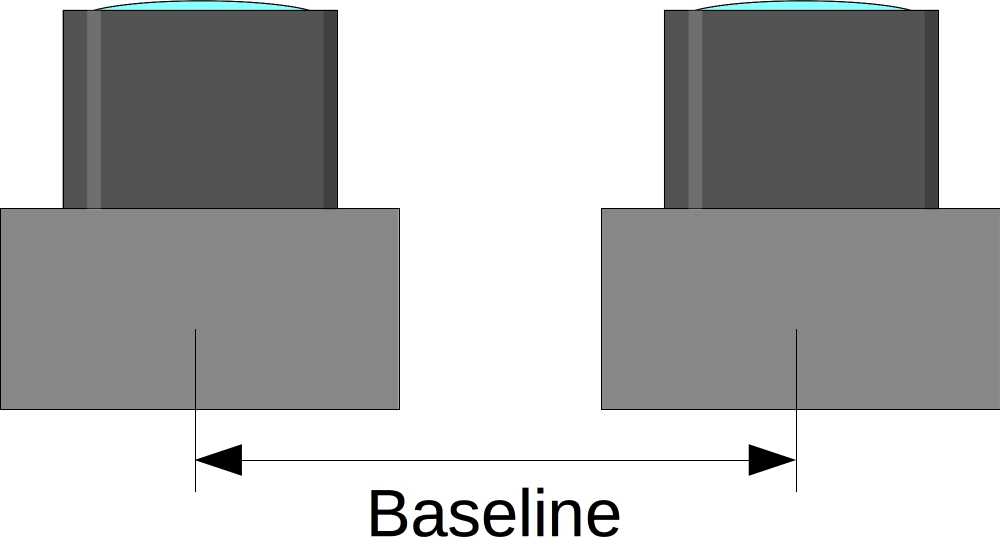
\includegraphics[width=0.5\textwidth]{figures/2cams_top}
    \caption{Seen from above\label{fig:2cams_top}}
  \end{subfigure}
  \caption{Illustration of stereo setup\label{fig:2cams_all}}
\end{figure}

Figure \ref{fig:imgplane_all} shows how a scene is seen by the camera, is inverted in the optical center and projected onto the image sensor in the camera. The original image plane is located at the position of the image sensor but it is inverted compared to scene captured. To simplified comparisons to the real world an image plane can be placed opposite of the optical center at the same distance from the center and this image plane will not be inverted.  

\begin{figure}[ht]
  \centering
  \begin{subfigure}[t]{0.3\textwidth}
    \centering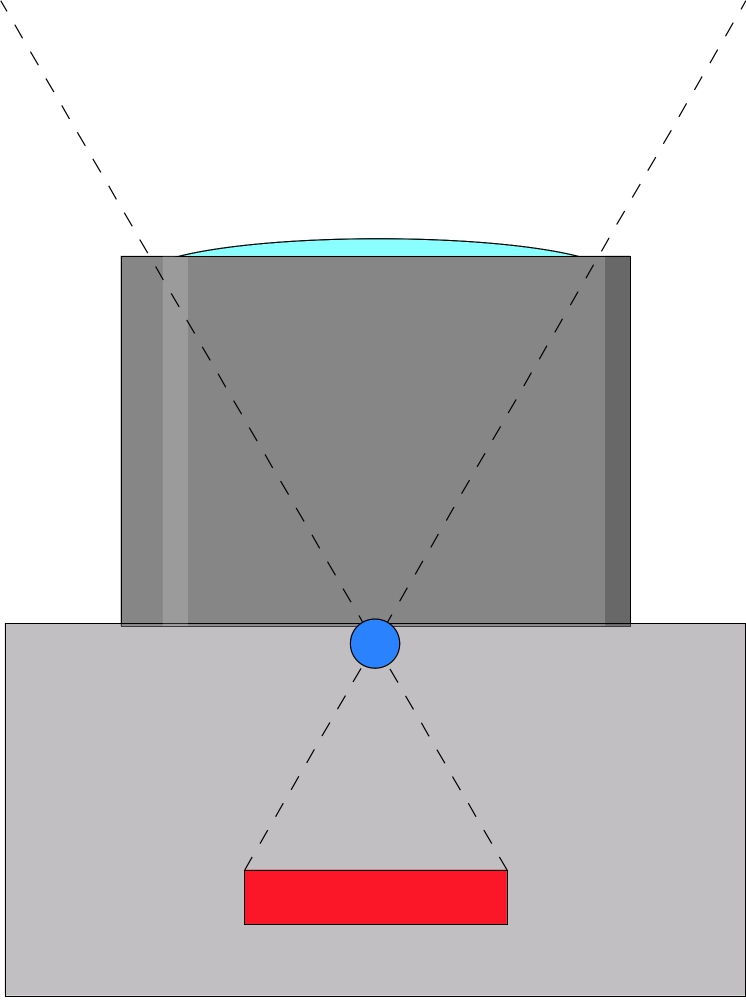
\includegraphics[height=4cm]{figures/imgplane_1.jpg}
    \caption{Location of the optical center and image sensor\label{fig:imgplane1}}
  \end{subfigure}\hspace{0.5cm}
  \begin{subfigure}[t]{0.3\textwidth}
    \centering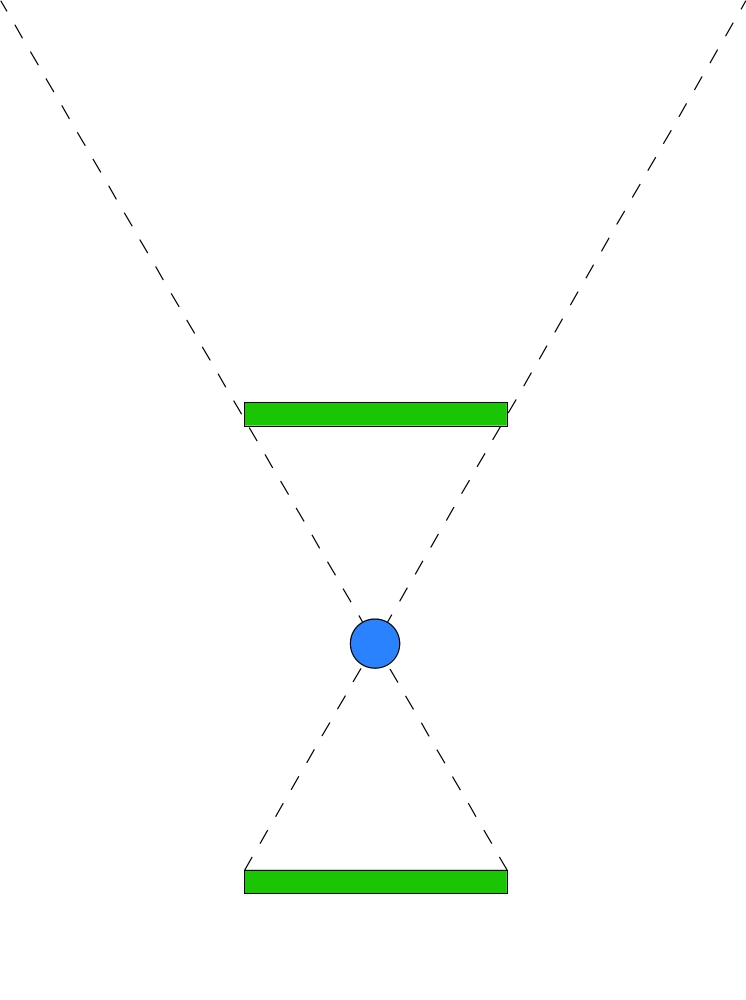
\includegraphics[height=4cm]{figures/imgplane_2}
    \caption{Location of the image plane\label{fig:imgplane2}}
  \end{subfigure}\hspace{0.5cm}
  \begin{subfigure}[t]{0.3\textwidth}
    \centering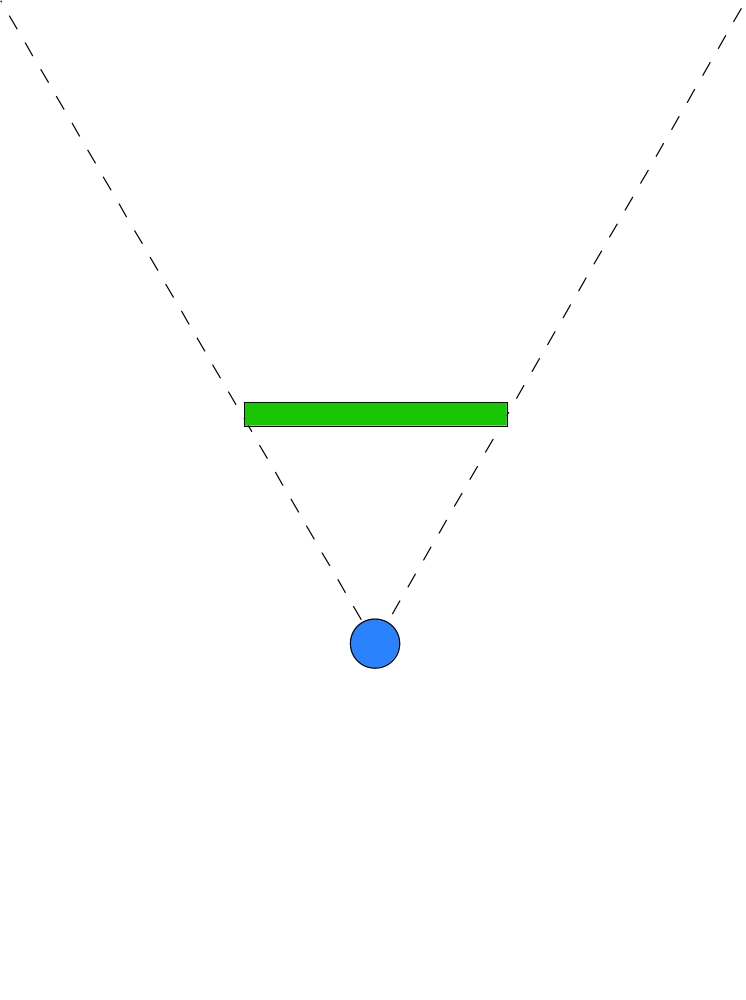
\includegraphics[height=4cm]{figures/imgplane_3}
    \caption{This illustration will be used to to explain disparity\label{fig:imgplane3}}
  \end{subfigure}
  \begin{subfigure}[t]{0.75\textwidth}
    \centering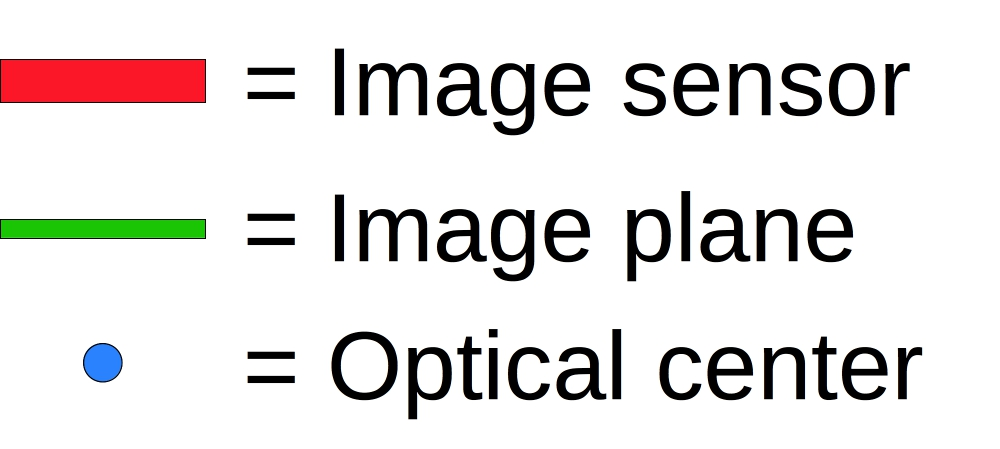
\includegraphics[width=0.4\textwidth]{figures/imgplane_legends}
  \end{subfigure}\hspace{0.5cm}
  \caption{Illustration of going from camera to image plane\label{fig:imgplane_all}}
\end{figure}

Figure \ref{fig:2points_1} shows that a single camera is not able to differentiate between two points at the same angle from the optical center but a different distance. Figure \ref{fig:2points_2} shows that adding the second camera shows that you then are able to differentiate between the two points.

\begin{figure}[ht]
  \centering
  \begin{subfigure}[t]{0.45\textwidth}
    \centering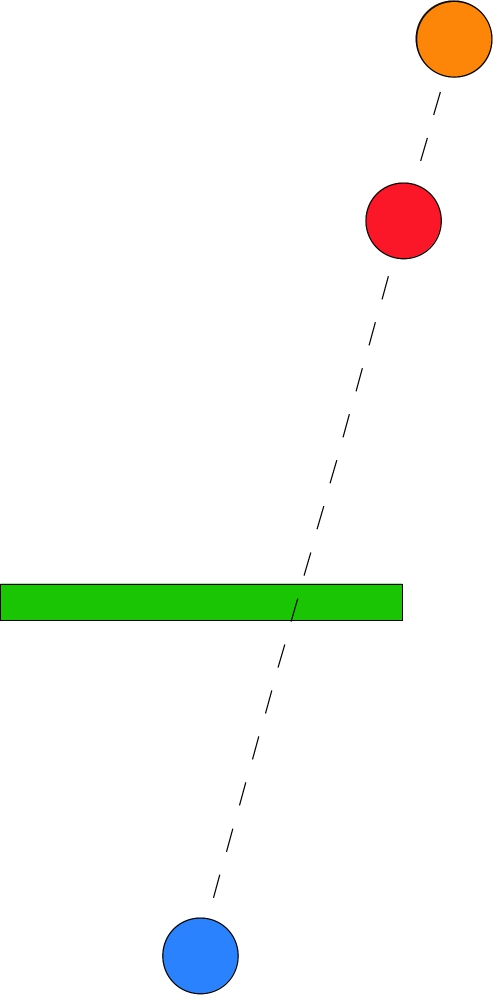
\includegraphics[height=4cm]{figures/2points_1}
    \caption{Seen from a single camera\label{fig:2points_1}}
  \end{subfigure}
  \begin{subfigure}[t]{0.45\textwidth}
    \centering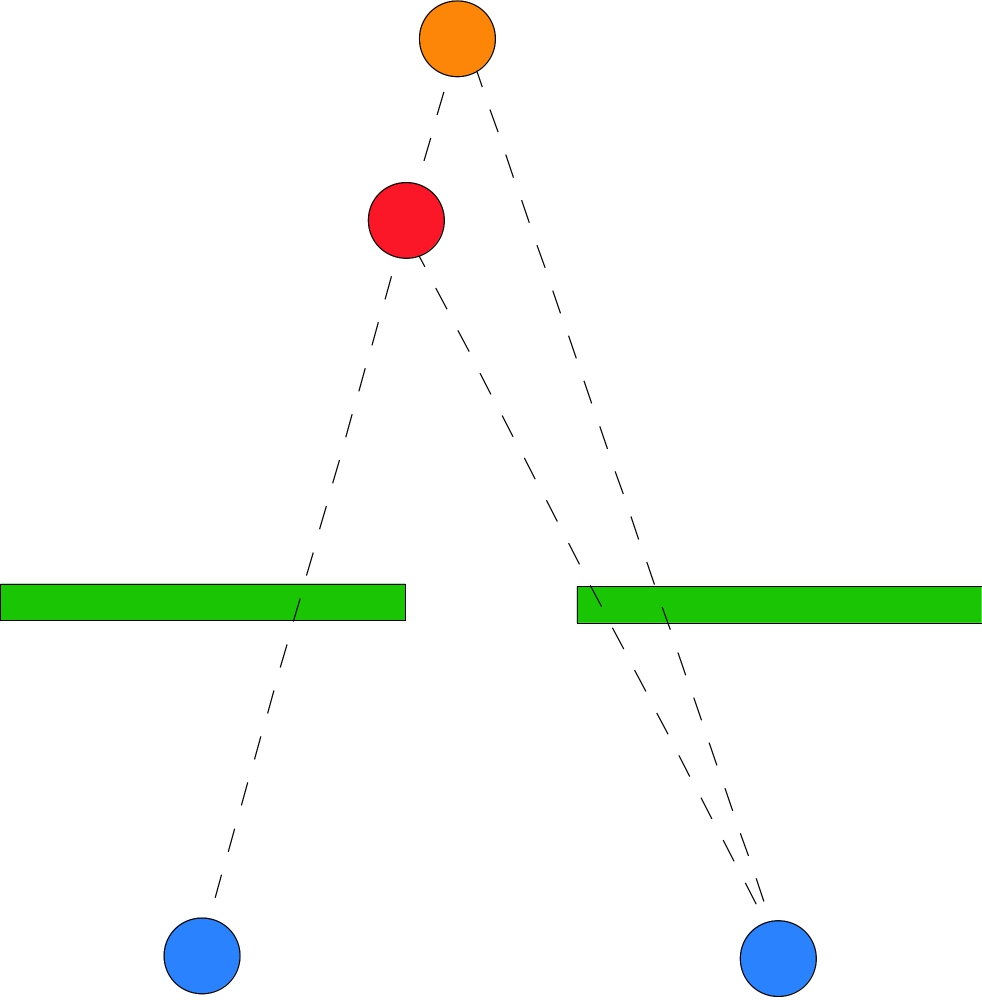
\includegraphics[height=4cm]{figures/2points_2}
    \caption{Seen from two cameras\label{fig:2points_2}}
  \end{subfigure}
  \caption{Example pf two points in a scene at different depths\label{fig:2points_all}}
\end{figure}

Figure \ref{fig:dispall} shows how the depth to a point can be calculated from the difference in x-positions on the image plane (the disparity). Figure \ref{fig:disp_long} and \ref{fig:disp_short} shows how the disparity change depending on the distance to the point. Two similar triangles can be created. One between the point, and the two optical centers. The other triangle is created between the point in the scene and the points where the dashed lines cross the image plane. Figure \ref{fig:bfz_disp} shows these two triangles and their heights. The small triangle have a height of $z$ and the bottom (the brown line) is equal to the baseline (purple line) minus the disparity and the large triangle have a height of $f+z$ and the bottom width is equal to the baseline. The ratio between the height and the bottom width is the same in the two triangles and hence the following equation can be formed:
\begin{flalign}
  && \frac{z+f}{b} &= \frac{z}{b-d} && \label{eq:disp_1} \\
  && z &= \frac{b \cdot f}{d} && \label{eq:disp_final}
\end{flalign}
\todo{ret denne formel til på et tidspunkt. \ref{eq:disp_final} er korrekt. Ændre den anden + måske figuren (z går vist fra baseline og ikke bare fra image plane)}

\begin{figure}[ht]
  \centering
  \begin{subfigure}[t]{0.3\textwidth}
    \centering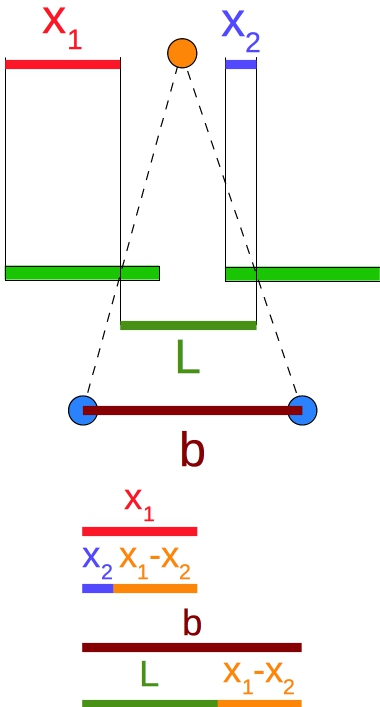
\includegraphics[height=5cm]{figures/disp_long.jpg}
    \caption{Disparity for a point far way\label{fig:disp_long}}
  \end{subfigure}\hspace{0.5cm}
  \begin{subfigure}[t]{0.3\textwidth}
    \centering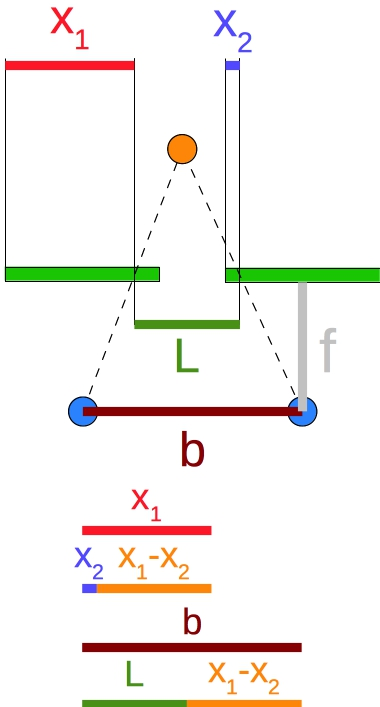
\includegraphics[height=5cm]{figures/disp_short}
    \caption{Disparity for point close\label{fig:disp_short}}
  \end{subfigure}\hspace{0.5cm}
  \begin{subfigure}[t]{0.3\textwidth}
    \centering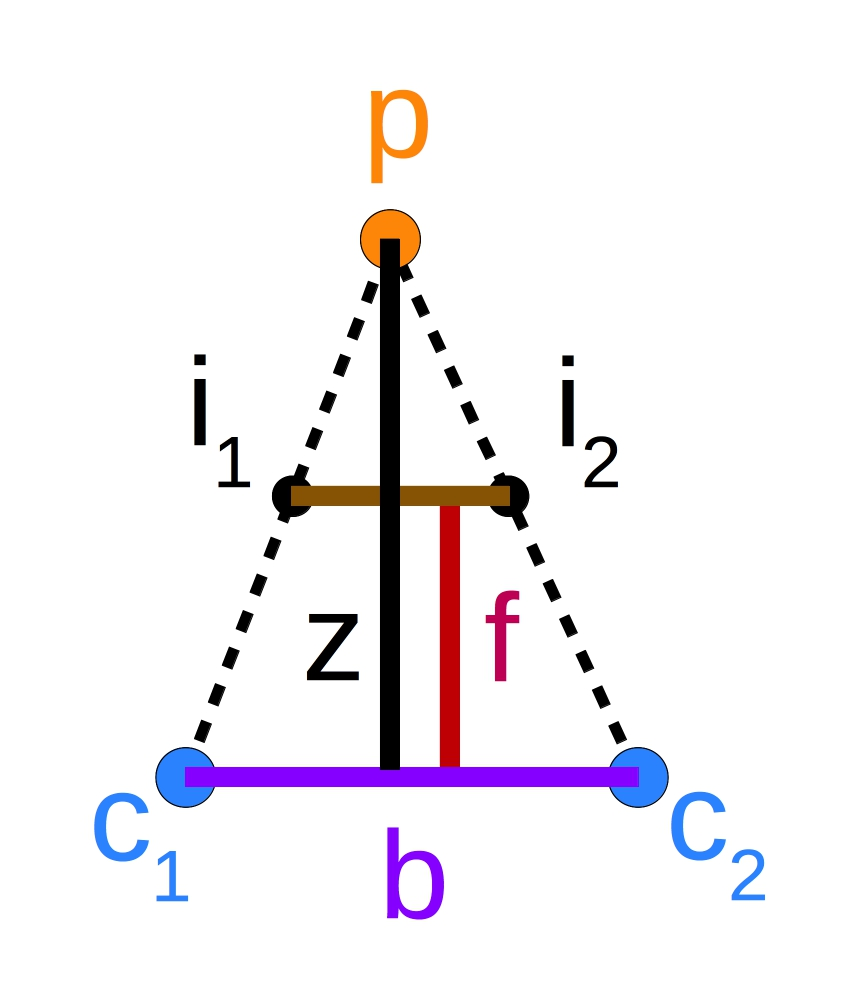
\includegraphics[height=5cm]{figures/bfz_disp}
    \caption{Illustration of triangles used for calculating the disparity\label{fig:bfz_disp}}
  \end{subfigure}
  \caption{Illustration of how to calculate depth from disparity\label{fig:dispall}}
\end{figure}

This explains the basic of stereo vision. The rest of this chapter will venture into other areals of stereo and describe the difficulties and solutions for each area.

\section{Rectification of stereo pairs}
The examples in section \ref{sec:basicstereo} uses ideal images to explain how stereo vision functions but in the real world the disparity is the difference along the epipolar lines which will have a different slope of each line and image. Different things can be done to simplify the search along epipolar lines. One thing is to rectify the stereo image pair. This will make all the epipolar lines horizontal and hence you only need to search along the x-axis.\\

The issue with rectification is that it is difficult to get a perfect match with the stereo setup since the every camera and its objective will be unique and require and all new manual adjustment. HSA system theorizes that a system can be developed which instead of rectifying the image it will find the epipolar lines and feed this information to the stereo camera. In this project stereo image pairs from Middlebury Vision Test set \cite{da} will be used which are rectified hence the rectification of image will not be researched further in this project.

\section{Color space and gray scale}
\todo{skriv noget om forskellige farve rum og grayscale og deres inflydelse på stereo algorithmen}
The article \textbf{Color correlation-based matching} takes the subject of difference in result when using color and which color space is used and grayscale when performing stereo matching. It performs different methods / algorithms using 9 different colorspace including grayscale. The result from the article is that color gives a better result with a few percentage of more correct estimations but the run time is much higher (ranging from 1.9 to 3.7 higher run time than grayscale on the teddy test set).
From this it is decided to not use color in case of Normalized Cross Correlation

\section{Resolution and disparity precision}
\todo{skriv noget om disparitets opløsning i forhold til billede opløsning osv.}

\section{Occlusion filling}
\todo{skriv noget om metoder til at udfylde occlusions områder}
This section will describe methods for filling the occluded areas. All these methods comes from the article: \textit{Occlusion filling in stereo: Theory and experiments} by \textit{Shafik Hyq, Andreas Koschan} and \textit{Mongi Abidi}. All these methods assume that the stereo matching is going from left image to right image i.e. templates are taken from the left image matched onto the right image.
 
\subsection{Neighbor's Disparity Assignment : NDA}
This is the simplest method to fill occlusions. It functions by selecting an occluded point, $p_L$, then find then nearest non-occluded point, $q_L$, to the left when filling non-border occlusion. With border occlusion the nearest point to the right is found instead. It is assumed that this non-occluded point is part of same surface as the occluded point (this can be seen on figure \ref{fig:borNParOcc}) and the disparity value from $q_L$ can be assigned to $p_L$. This method have some issues. In cases of total occlusions (see figure \ref{fig:totalOcc}) then a wrong disparity value is given to the total occluded object since it isn't a part of the nearest surface with non-occluded points to the left. In cases with self occlusions the occluded area should have disparity values close to the disparity values of the non-occluded points to the right (This will be the area of the surface which is in view of both cameras) but using NDA will give the occluded area disparity values corresponding to the background. 

\subsection{Diffusion in Intensity Space : DIS}
This method is inspired by diffusion. Diffusion is the movement of molecules or atoms from a high concentration region to a low concentration region. \\
After detecting occluded regions with cross-checking during template matching, the diffusion energy for the region is approximated. This method is depended on the stereo matching algorithm because it use the energy from the last iteration to determine initial diffusion energy for the area. \\
A change to the method can be made to make it independent from the stereo matching. The initial energy will be 0. Then the diffusion energy for non-border occlusion is found by:
\begin{equation}
E(p_L) = \min_{l_{p_L}=\{0,\dots, l_{max}\}} \left( \dfrac{1}{2 | q_L \in \mathcal{N}(p_L) \wedge l_{q_L=l_{p_L}} |} \; \sum_{q_L \in \mathcal{N}(p_L) \wedge l_{q_L = l_{p_L}}} (|\bar{I}(p_L)-\bar{I}(q_L) | + E(q_L))\right)
\end{equation}
And the diffusion energy for border occlusions are found by by:
\begin{equation}
E(p_L) = \min_{l_{p_L}=\{0,\dots, l_{p_{Lf}}-2\}} \left( \dfrac{1}{2 | q_L \in \mathcal{N}(p_L) \wedge l_{q_L=l_{p_L}} |} \; \sum_{q_L \in \mathcal{N}(p_L) \wedge l_{q_L = l_{p_L}}} (|\bar{I}(p_L)-\bar{I}(q_L) | + E(q_L))\right)
\end{equation}
The diffusion energy will be calculated for each occluded point and for each point the disparity which corresponds the minimum $E(p_L)$ is set as the disparity $l_{p_L}$ for the occluded point. 


\subsection{Weighted Least Squares : WLS}
In this approach, WLS, all the non-occluded and filled occluded neighbors in a neighborhood around the occluded point is considered valid points and is used as control points in interpolation.\\
Since the neighborhood contains both foreground points and background points and the occluded point is expected to be a part of the background then the background points should have more influence than foreground points. It is assumed that the color intensity between objects is significantly different and this property can be used to distinguish between foreground points and background points. \\
Each error term in the aggregated residual should be weighted so the foreground don't have much influence. With this the aggregated residual is defined as:
\begin{equation}
  \Delta = \sum_{q_L \in \mathcal{N}(p_L)} w_{q_L} (\hat{l}_{p_L}(p_L)-l_{p_L}(q_L))^2
\end{equation}
where $w_{q_L} = e^{-\mu_L | \bar{I}(p_L) - I(q_L)|}$ (the weight) is the likelihood of $p_L$ with $q_L$ under the assumption of an exponential distribution model of $| \bar{I}_(p_L)- I(q_L) |$. $\bar{I}(p_L)$ is the mean intensity of $p_L$ and $\mu_L$ is the decay rate. $\hat{l}_{p_L}(p_L)$ is the estimated disparity of $p_L$ (will be estimated during interpolation) and $l_{p_L}(q_L)$ is the disparity of $q_L$. \\
How to estimate $\bar{I}(p_L)$ and $\mu_L$:\\
$\bar{I}(p_L)$ is the mean intensity of $p_L$ which can be obtained using mean shift algorithm in a window around $p_L$. To estimate this value the initialize the algorithm with $\bar{I}(p_L) $ equal to the intensity of $p_L$ then the mean shift algorithm repeatedly picks those neighbors inside the window that satisfy $| \bar{I}(p_L) - I (q_L) | \geq 3\mu^{-1}$ and the assign the average of intensities of the selected neighbors to $\bar{I}(p_L)$ until $\bar{I}(p_L)$ converges to a fixed average. $|\bar{I}(p_L) - I(q_L)|$ has decay rate $\mu_L$ which is related to the decay rate $\mu$ of the variable $|I(p_L) - I(q_L)|$ by $\mu_L^2 = \mu$.\\
A matrix containing all the coordinates:
\begin{equation}
F = \begin{bmatrix}
  x_1 & y_1 & 1 \\
  \vdots & \ddots & \vdots\\
  x_n & y_n & 1 
\end{bmatrix}
\end{equation}
Vector with the corresponding labels for the coordinates in $F$:
\begin{equation}
L = [l_1 \; \cdots \; l_N] 
\end{equation}
Linear model:
\begin{equation}
l_{p_L} = a + b x (p_L) + c y (p_L)
\end{equation}
Where $(x(p_L),y(p_L))$ is the coordinates of $p_L$ and $a$, $b$ and $c$ are the model parameters. \\
The weights for the control points can be express in a vector as:
\begin{equation}
w = [w_{q_{L1}} \; w_{q_{L2}} \; \cdots \; w_{q_{LN}}]'
\end{equation}
Then we compute two new matrices, $F_w$ and $L_w$:
\begin{flalign}
&& F_w &= diag(w)F && \\
&& L_w &= diga(w)L &&   
\end{flalign}
The model parameter vector:
\begin{equation}\label{eq:parvec}
P = [\, a \; b \; c \,]'
\end{equation}
By combining the equations above then the following equation is given: 
\begin{equation}
P = (F^T_wF_w)^{-1}F^T_wL_w
\end{equation}
With these equation the disparity of the occluded point can be estimated:
\begin{equation}
\hat{l}_{p_L} = [1 \; x(p_L) \; y(p_L)] P
\end{equation}

\subsection{Segmentation-based Least Squares : SLS}
Biggest difference between WLS and SLS is that SLS only uses non-occluded points as control points. The control points is a subset of the non-occluded neighboring points. The control points are segmented from the neighborhood by applying different constraints: visibility constraint, disparity gradient constraint and color similarity cues. \\
Sequence of operations: 
\begin{itemize}
\item Select an occluded point
\item Select control points from the neighborhood around the occluded point
\item Interpolate the disparity of the occluded point from the segmented control points 
\end{itemize}
$\mathcal{N}(p_L)$ is a set of non-occluded, neighboring points which will be use for control points in the interpolation. For points to be added to $\mathcal{N}$ then it needs to fulfill some constraints.\\
\textbf{Disparity gradient constraint:} In most cases the horizontal closest non-occluded point to the right, $p_{Lf}$, will be part of the foreground and the occluded should be a part of the background. In this cases every non-occluded point with a lower disparity than $p_{Lf}$ will be added to $\mathcal{N}$ hence the condition for added the point, $q_L$, will be $l_{q_L} < l_{p_{Lf}}$. If the foreground object is narrow then all the non-occluded neighboring points might be from the background and have the same disparity. Due to this a second condition have to be added to the constraint. The horizontal closest non-occluded point to the left will be called $p_{Lb}$ and a second condition is created: $| l_{p_{Lb}} - l_{q_L} | \leq 1$. When these conditions are combined the constraint can be defined as:
\begin{equation}
| l_{p_{Lb}} - l_{q_L} | \leq 1 \vee  l_{q_L} < l_{p_{Lf}}  
\end{equation}
\textbf{surface constraint:} It is assumed that $\mathcal{N}(p_L)$ will contain points from maximum 2 different surfaces (due to the small neighborhood). Some cases might contain a third surface but this is expected to occur very seldom and therefore it is disregarded. The point with the lowest disparity, $l_{min}$, is assumed to belong to one of the surfaces and the point with the highest disparity, $l_{max}$, is assumed to belong to the other surfaces. If $l_{max} - l_{min} \leq 1$ then it is assumed the all the points in $\mathcal{N}$ belongs to a single surfaces otherwise the points have to be segmented into 2 groups. The first group will contain all points which satisfies $| l-{max} - l_{q_L} | \leq 1$ and the other group will contain all the points which satisfies $| l-{min} - l_{q_L} | \leq 1$.
\textbf{Color constraint:} The average truncated color distance from the occluded point, $p_L$, to each of the two groups to determine which group the point belongs to. The average truncated color distance is found by:
\begin{equation}
D(p_L,\mathcal{N}_i(p_L) ) = \dfrac{1}{|\mathcal{N}_i(p_L)|} \; \sum_{q_L \in \mathcal{N}(p_L)} \psi (p_L,q_L) 
\end{equation}

\section{Mini-conclusion}
\todo{find på et bedre navn til denne sektion}
To conclude this chapter the findings for each area in stereo vision will be examined and it will be specified which solution will be used from this point.
\subsection*{•}

\chapter{Design and test specification} \label{ch:req}
This chapter elaborates on the requirements for the system and derives a test specification which will describe how to test for the requirements.\\

A way to identify the performance of a design using different design metrics is the cost function. The cost function specifies the overall cost of a design and is a function of the different design metrics:
\begin{equation}
C = f(A,T,P,N,test) = a_1\cdot A + a_2 \cdot T + a_3 \cdot P + a_4 \cdot N + a_5 \cdot S
\end{equation}
where $A$ is area, $T$ is time, $P$ is power, $N$ is numerical properties, $S$ is the stereo matching result from Middlebury test and $a_i$ tells the importance of the associated metric.\\
It is the task of the system designer to minimize this cost. And due to $a_i$ the cost function can be changed to fit the priorities of the application.\\

For this thesis, the number one priority is the time metric since it is required that the algorithm should be executable in real-time. The stereo matching metric is also important since it describes the quality of the resulting disparity map i.e. the number false disparity values. Numerical properties are 3rd most important metric since this can affect the result from the algorithm since the cost value may have added noise. Area is not as important because if the target FPGA is too small then HSA Systems will use a larger FPGA but larger area often equals more expensive hardware. Power isn't important either since the stereo setup is intended being a part of industrial systems hence power is easily accessible.\\

An ordered list of priorities for the design metrics in this project:
\begin{multicols}{2}
  \begin{enumerate}
    \item Time
    \item Stereo matching result
    \item Numerical properties
    \item Area 
    \item Power\\~\\
  \end{enumerate}
\end{multicols}

In this thesis, the cost function will be used when choosing e.g when comparing the different algorithms found in chapter \vref{ch:alganalysis}.

\section{Requirement specification}
This section will contain a table with the requirements for the system. Each parameter will be given a number, a value which should be met, the unit for the value, additional information for the requirement and a reference to where discussion for the requirement can be found.
\begin{table}[ht!]
  \centering
  \begin{tabular}{l m{2cm} c c m{5cm} m{1.9cm}}
  \toprule
  \textbf{No.} & \textbf{Parameter} & \textbf{Value} & \textbf{Unit} & \textbf{Additional Information} & \textbf{Source} \\
  \midrule
  1 & Frame rate & $\geq 10$ & fps & & Section \vref{req:framerate} \\
  \midrule
  2 & Disparity precision & $\leq 5$ & \si{\milli\meter} & \tabitem Either directly or using \newline \hspace*{0.4cm}subpixel refinement \newline \tabitem In the range 0.5-\SI{1.5}{\meter}  & Section \vref{req:dispre}\\
  \midrule
  3 & Camera resolution & 2464$\times$2056 & pixels & & Section \vref{req:camres} \\
  \midrule
  4 & Pixel size & \num{3.45} & \si{\micro\meter} & & Section \vref{req:pixelsize} \\  
  \midrule
  5 & Focal length & \num{7.09} & \si{\milli\meter} & & Section \vref{req:focallen} \\
  \midrule
  6 & Scene size & \num{1.5}$\times$\num{1.5} & \si{\meter} & & Section \vref{req:scenesize} \\
  \toprule
  \multicolumn{6}{l}{The algorithm should be implemented on a \textit{Xilinx Zynq Z7020}}\\
  \bottomrule
  \end{tabular}
\end{table}

\section{Test specification}
This section will describe how the system can be tested in order to ensure that the requirements are fulfilled. \\

Requirement 1: frame rate can be tested by running the finalized implementation and measure the run time which then should be \SI{\leq 100}{\milli\second}. \\

Requirement 2: disparity precision. This requirement can be tested if a working stereo camera setup is developed. \\
HSA Systems has produced a depth precision test object with small depth differences. The object is shown on figure \vref{fig:3dpreobj}. The object consists of five sets of steps with each stair having different depth increment. Looking at \vref{fig:3dpretestpic} the set of steps in the bottom have a depth difference of \SI{5}{\milli\meter} between each step. The set of steps just above have a depth difference of \SI{4}{\milli\meter} between each step. This pattern continues and results in the top set of steps to have a depth difference of \SI{1}{\milli\meter}. The small shapes in the middle of each steps have a depth difference of \SI{0.5}{\milli\meter} alternately protrude from or recess into the steps.\\

\begin{figure}[ht]
  \centering
  \begin{subfigure}[t]{0.45\textwidth}
    \centering\raisebox{22.25mm}{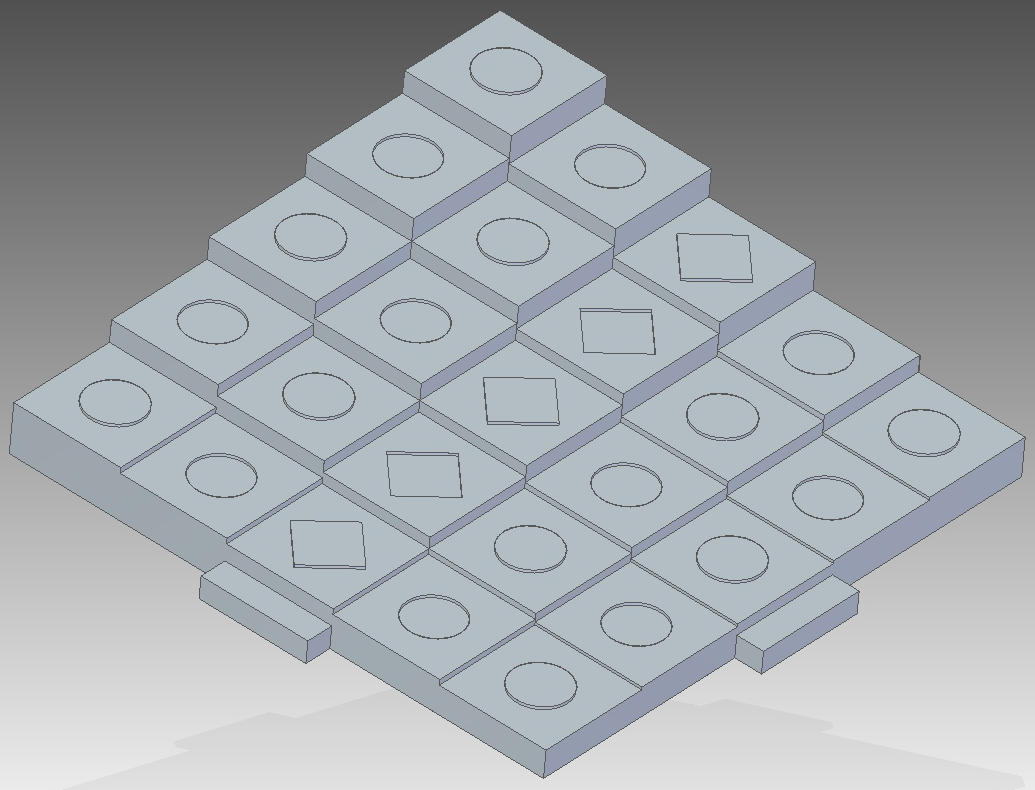
\includegraphics[width=0.9\textwidth]{figures/3dprecisiontest}}
    \caption{3D model of depth precision test object}
    \label{fig:3dpretest}
  \end{subfigure}\hspace{0.5cm}
  \begin{subfigure}[t]{0.45\textwidth}
    \centering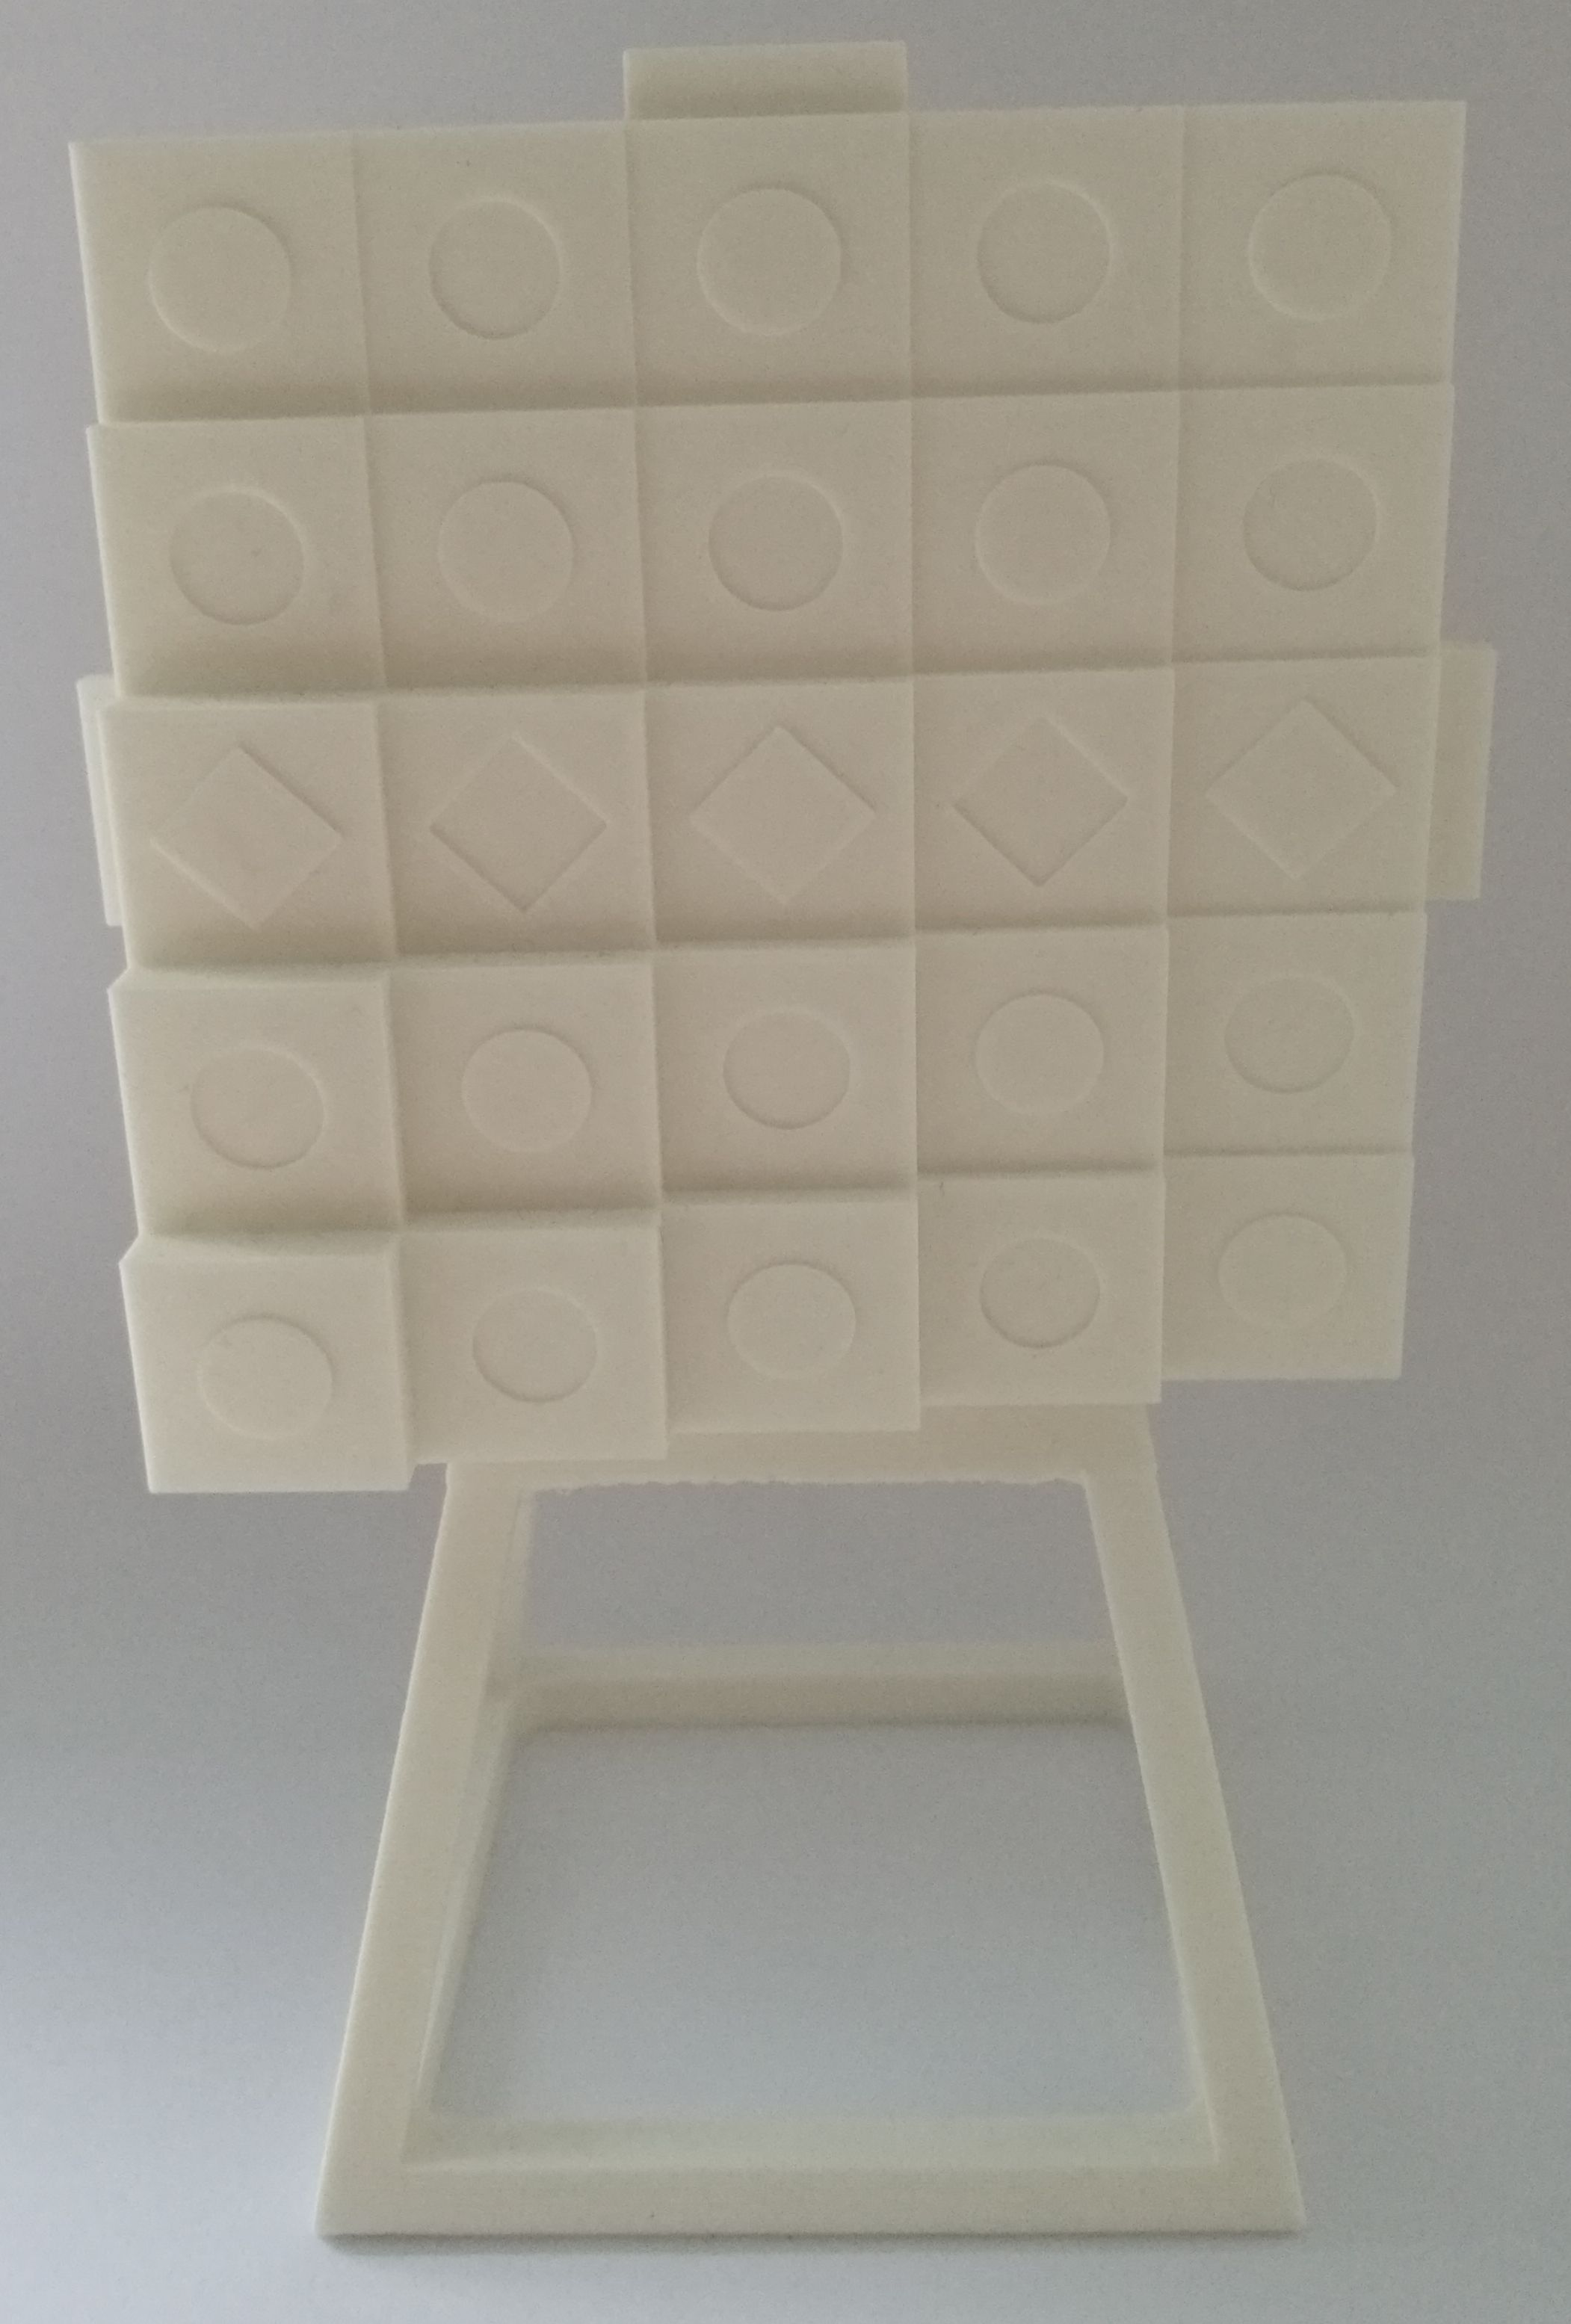
\includegraphics[width=0.9\textwidth]{figures/testobject_foot}
    \caption{Picture of 3D printed depth precision test object}
    \label{fig:3dpretestpic}
  \end{subfigure}
  \caption{Depth precisison test object \label{fig:3dpreobj}}
\end{figure}
Placing this object at a specific distance the depth precision can be tested. If the steps in lowest set of steps can be distinguish from each other in the disparity map then the depth precision is \SI{\leq 5}{\milli\meter}.\\
If the implementation can distinguish between the lowest set of steps and the object is placed at \SI{1.5}{\meter} from the camera setup then the requirement is fulfilled. The rest of the steps help determine if the camera have a better precision than required.\\
The middlebury test set does not contain images where specific areas contain depth increments of 2 mm and therefore these images can not be used for testing this requirement and calculations \vref{sec:disppre} are used instead.\\

Requirement 3: camera resolution is fulfilled by choosing the correct camera hardware but is essential to be fulfilled for requirement 2 to be fulfilled.\\

requirement 4: pixel size is fulfilled by choosing the correct camera hardware but is essential to be fulfilled for requirement 2 to be fulfilled.\\

requirement 5: focal length is fulfilled by choosing the correct camera hardware but is essential to be fulfilled for requirement 2 to be fulfilled.\\

Chapter \vref{ch:acctest} will perform the available tests.


\chapter{Algorithm design}
\todo{ROUGH SKETCH not done yet}

In this chapter the two stereo vision algorithms, Efficient Edge Preserving Stereo Matching (EEPSM) and Fast Cost-Volume Matching (FCV), is described. Lastly, a simulation of each algorithm is created and the results of these simulations are compared and from this, an algorithm is chosen.

\section{Efficient Edge Preserving Stereo Matching:}
This algorithm works in three steps. The first step is calculating a cost for each pixel and disparity. This cost is a combination of the sum of absolute differences and hamming distance of the census transform around each pixel.
\begin{flalign}
&& C^{SAD}_d(x,y) &=  \sum^3_{i=1}| I_{left}(x,y,i) - I_{right}(x+d,y,i) |  &&\\
&& C^{CENSUS}_d(x,y) &= Ham(CT_{left}(x,y),CT_{right}(x+d,y)) && \\
&& C_d(x,y) &= \alpha \cdot C_d^{SAD} (x,y) + (1-\alpha)\cdot C^{CENSUS}_d (x,y) &&
\end{flalign}
where $d$ is the disparity estimate, $I_{left}$ is the left image, $I_{right}$ is the right image, $i$ is the color (rgb), $Ham(x_1,x_2)$ is the hamming distance between $x_1$ and $x_2$, and $CT_{left}$ and $CT_{right}$ is the census transform around the specified pixel\\
then a permeability weight is calculated. Permeability is known from biomedicine and describes the ability to transfer through a membrane. The permeability weight is inspired by this and describes how well the color transfers from one pixel to another pixel. 
\begin{flalign}
  && \mu(x,y) &= \min(e^{\frac{-\Delta R}{\sigma}},e^{\frac{-\Delta G}{\sigma}},e^{\frac{-\Delta B}{\sigma}}) &&\\
  && \mu_{tb}(x,y) &= \min(e^{\frac{-(R(x,y)-R(x,y-1))}{\sigma}},e^{\frac{-(G(x,y)-G(x,y-1))}{\sigma}},e^{\frac{-(B(x,y)-B(x,y-1))}{\sigma}}) &&
\end{flalign}
lastly, the cost is aggregated resulting in a combined cost for each pixel at each disparity. The cost from equation ?? is first aggregated horizontally using permeability weights from equation ??. Then the result from horizontal aggregation is aggregated vertically also using the permeability weight. 

\begin{flalign}
  && C_d^{lr}(x,y) &= C_d(x,y) + \mu_{lr}(x,y) \cdot C_d(x-1,y) &&\\
  && C_d^{lr}(x,y) &= C_d(x,y) + \sum_{i=1}^{x-1} \left(C_d(x-i,y) \cdot \Pi_{j=i}^{i} \mu_{lr}(x-1,y) \right) &&
\end{flalign}

With a cost at each pixel at each disparity estimate, the disparity map can be generated by minimization along the disparity estimates.

\section{Fast Cost-Volume Matching:}
This algorithm starts by calculating a cost for each pixel at each disparity estimate. This cost consists of the sum of absolute differences and differences in the gradient.

\begin{flalign}
 && C^{SAD}_{d} (x,y) &= \sum^3_{i=1}| I_{left}(x,y,i) - I_{right}(x+d,y,i) |  &&\\
  && C^{Grad}_{d} (x,y) &= \nabla_x I_{left}^{g} (x,y) - \nabla_x I_{right}^{g} (x,y) &&\\
  && C_{d} (x,y) &= \alpha \cdot C^{SAD}_{d} (x,y) + (1 - \alpha) \cdot C^{Grad}_{d} (x,y) &&
\end{flalign}  

These cost values are then filtered using a Guided Image Filter. The guided image filter is a filter uses a reference image to generate the weights. The guided image filter is described further in section \ref{sec:guidedif}

\begin{flalign}
  && C'_d (x,y) &= \sum_j W_i,j(I)C_d(x,y) &&
\end{flalign}

The correct disparity for each pixel can then be found by minimizing along the disparity estimates as seen in equation \ref{eq:fcvmin}.

\begin{flalign} \label{eq:fcvmin}
  && f(x,y) &= \arg \min_{d \in [0,d_{max}]} C'_d(x,y)&&
\end{flalign}

\subsection{Guided image filter} \label{sec:guidedif}
The guided image filter uses a image as a reference for weighting the input. The output from the filter is seen in equation  

\begin{flalign}
  && q_i &= \sum_j W_{i,j}(I)p_j &&\\
  && q_i &= a_k I_i + b_k \quad, \forall i \in \omega_k &&
\end{flalign}
where:
\begin{flalign}
  && a_k &= \dfrac{\frac{1}{|\omega|} \sum_{i \in \omega_k} I_i p_i - \mu_k \bar{p}_k}{\sigma^2_k + \epsilon} &&\\
  && b_k &= \bar{p}_k - a_k \mu_k &&  
\end{flalign}

\subsubsection*{algorithm}
\textbf{Input:} \\
filtering input image: $p$\\
guidance image: $I$\\
radius: $r$\\
epsilon: $\epsilon$\\
\textbf{Output:} \\
filtering output: $q$\\
\textbf{Steps:}
\begin{enumerate}
  \item $\mu_I = f_{mean}(I)$ \\
           $\mu_p = f_{mean}(p)$ \\
           $\rho_{II} = f_{mean}(I \cdot I)$ \\
           $\rho_{Ip} = f_{mean}(I \cdot p)$
  \item $\sigma_I = \rho_{II} - \mu_I \cdot \mu_I$\\
           $cov_{Ip} = \rho_{Ip} - \mu_I \cdot \mu_p$
  \item $a = cov_{Ip}/(\sigma_I + epsilon)$\\
           $b = \mu_p - a \cdot \mu_I $
  \item $\mu_a = f_{mean}(a)$\\
           $\mu_b = f_{mean}(b)$
  \item $q = \mu_a \cdot I + \mu_b$
  
\end{enumerate}

\section{Simulation and comparison}
\todo{simulation af de 2 algorithmer og samlign resultaterne.}

\section{Choosing an algorithm}
\todo{Nok en anden titel til denne sektion. Skriv hvilken algorithme jeg går videre med}

\chapter{Platform analysis} \label{ch:plaanalysis}
This chapter the hardware platform provided for this is described. For this project, HSA systems have provided a Zedboard Development Board \cite{Zedboard2014}. This board is used for this project since it contains a Zynq Z-7020 SoC from Xilinx, which HSA Systems uses for multiple products. 
\begin{figure}[ht!]
  \centering
  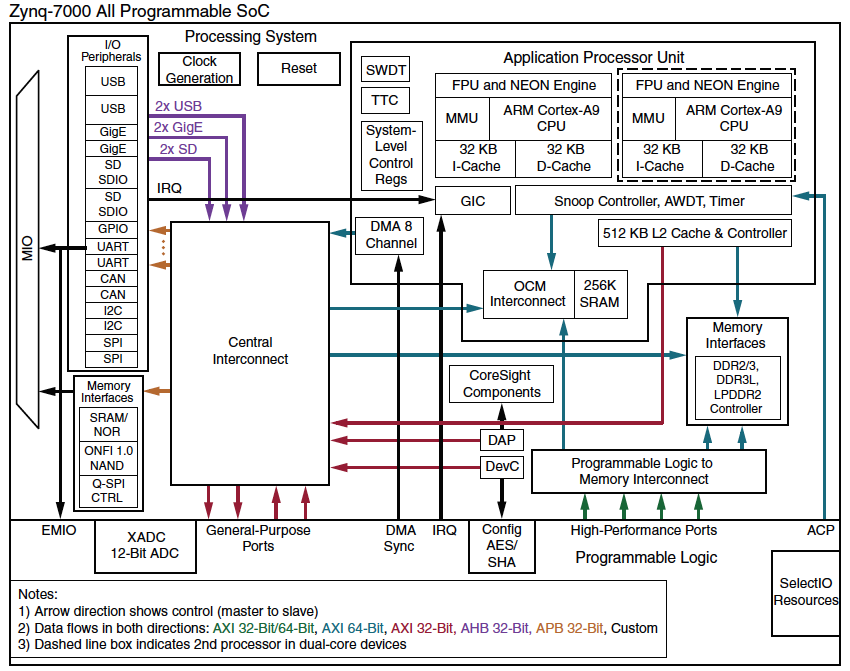
\includegraphics[width=0.75\textwidth]{figures/z7020overview}
  \caption{Architectural Overview \cite{zynq20137000}}
  \label{fig:z7020over}
\end{figure}
The Zynq SoC contains an ARM$^\text{\textregistered}$ Processing system and 7 series programmable logic (FPGA). This thesis project will focus on the programmable logic of Zynq SoC. Figure \vref{fig:z7020over} shows an overview over the Zynq Z-7000 architecture. From this figure it can be noticed that the \textit{programmable logic} is located at the bottom and all the connection to the rest of the system is seen. In the upper right of the overview, the ARM$^\text{\textregistered}$ cores are located. In this project the GPP part of the SoC will be used of OS and likewise assignments. The algorithm will mostly be implemented in the programmable logic.

\begin{table}[ht!]
  \centering
  \begin{tabular}{l c}
  \toprule
  \textbf{Part} & \textbf{Quantity} \\
  \toprule
  Programmable logic cells &  85,000\\
  \midrule
  Look-Up Tables & 53,200\\
  \midrule
  Flip-flops & 106,400\\
  \midrule
  Block Ram  & 4.9 Mb\\
  \midrule
  Programmable DSP slices & 220 \\
  \bottomrule
  \end{tabular}
  \caption{Programmable logic - Zynq 7020 \cite{zynq20137000}}
  \label{tb:z7020-parts}
\end{table}

Text about platform trade-off\\
When designing embedded systems the choice of platform is important. Different platform exists each with their own advantages and disadvantages. Figure \vref{fig:plattrade} illustrates the relation between design time and flexibility for general platform types. \\
\begin{figure}[ht!]
  \centering
  %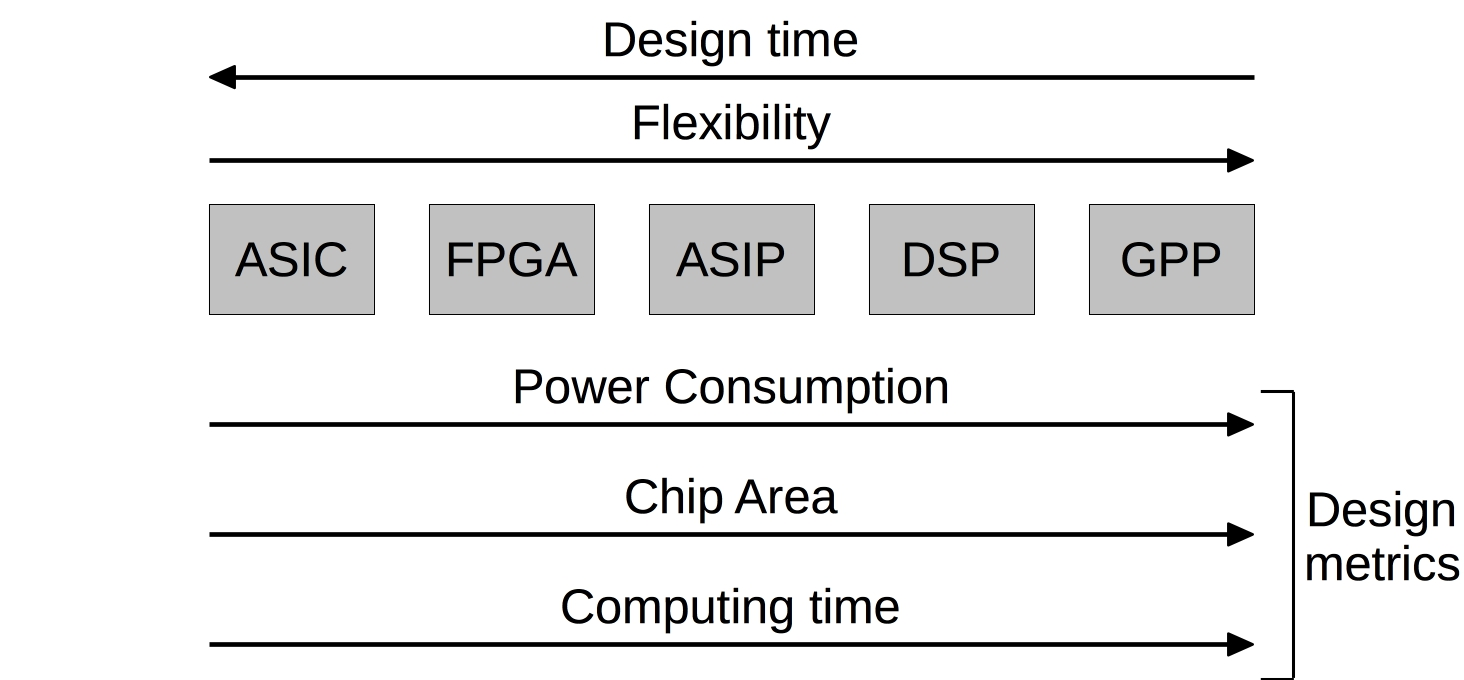
\includegraphics[width=0.7\textwidth]{figures/plattrade2}
  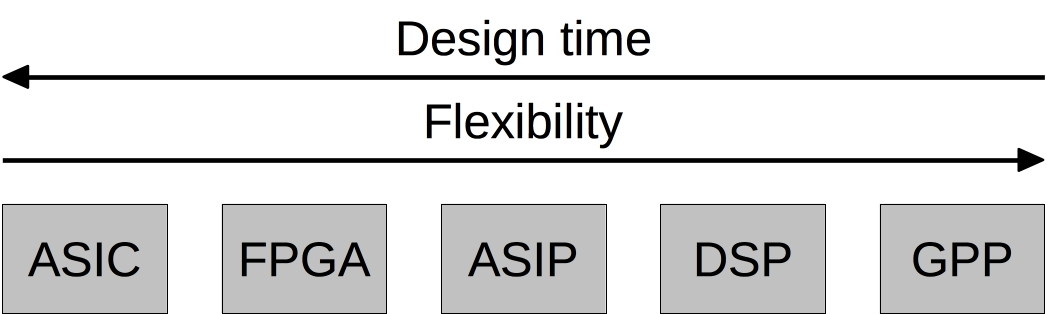
\includegraphics[width=0.5\textwidth]{figures/plattrade}
  \caption{Relation between design time and flexibility for general platform types.}
  \label{fig:plattrade}
\end{figure}
From this figure it is seen that there is a clear trade-off between a general-purpose processor (GPP) and an application specific integrated circuit (ASIC). The other platforms fall in between these two, in terms of the metrics. \\

A GPP is a popular choice due to its short design time and high flexibility. It is optimized for data manipulation, control flow and sequential performance. However in the area of signal processing applications  

\section{Hardware utilization}
In this section, the hardware utilization of the Xilinx Vivado software and the Zedboard is explored. The software used is the Vivado HL Design Edition 2016.2. To get a simple approximation of the hardware utilization some simple systems have been generated in the software and synthesized and implemented. Simple systems with a specified functional unit have been created using the Block Design system in Vivado. 100 copies of the specified functional unit were added. 
\begin{figure}[ht!]
  \centering
  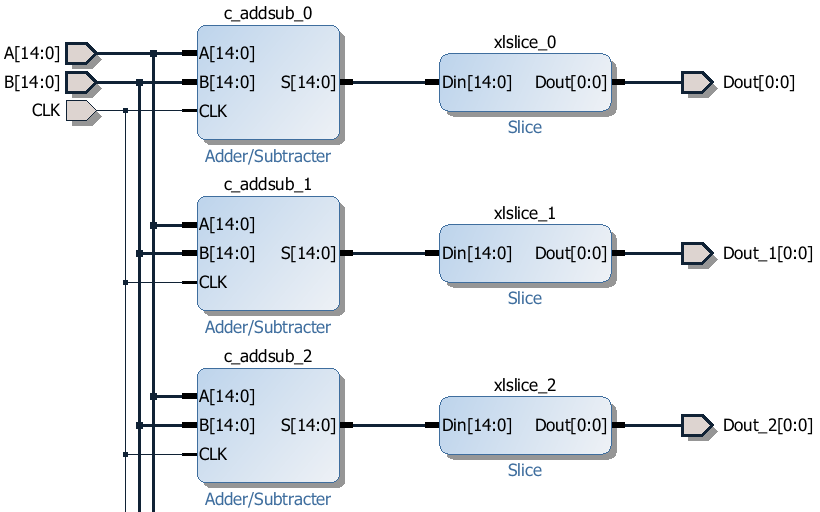
\includegraphics[width=0.75\textwidth]{figures/Blockdesignexample.png}
  \caption{Example of block design in vivado}
  \label{fig:blodesexa}
\end{figure}
The reasoning for 100 copies is to ensure that the contribution from control signals and wiring is minimized. With a block design generated it can be synthesized. In Vivado there are 2 steps. The first step is \textit{synthesize} where the software figures out which hardware is needed for the system and then the next step is \textit{implementation} where the software optimize the hardware use for the platform it is implemented on. To complete the \textit{implementation} step then the design have to fit the target hardware so the design must not exceed the number of available I/O ports etc. When generating the block design IP blocks from Xilinx was used and for most FUs inputs and outputs of 16 bits where used. Each output needs to be connected to its own port and this will result in the implementation step to fail since too many I/O ports is used. Connecting the outputs to temporary signals and not using these signals will result in the \textit{implementation} step to optimize and remove all the adders since the output aren't used. Instead,  a Slice IP can be used to strip every bit but MSB. This results in every block only having an output size of \SI{1}{\bit} and the I/O usage have been lowered enough for the \textit{implementation} to succeed. Then the hardware utilization can be found in the software. These values are then divided by 100 to get a rough idea of how much hardware each functional unit requires.\\
Appendix~\vref{app:alloctest} describes more thoroughly the procedure for these tests and table~\ref{tab:utilizationofelements} shows the result.
\begin{table}[ht!]
\centering
\begin{tabular}{l | c c c c }
  \toprule
   &  LUT & FF & BRAM & DSP48 \\
  \midrule
  Adder & 15 & 15 & - & - \\
  Adder/Subtracter  & $\approx 16$ & 15 & - & - \\
  Subtract  & 15 &  15 & - & - \\
  Multiplier - LUT  & 352 &  36 & - & - \\
  Multiplier - DSP48 & - & - & - & 1 \\
  Divider & $\approx 177$ & 82 & 0.5 & 7 \\
  \bottomrule
\end{tabular}
\caption{Number of logic elements used in average for each FU}
\label{tab:utilizationofelements}
\end{table}


\chapter{Design methodology}
\todo{læs om system design methodologies i gajski's \textbf{Embedded Systems Design - Modeling, Synthesis and Verification} og beskriv Platform Methodology}

\chapter{Architecture design}
\todo{NOT DONE! rough sketch}

\section{Box filter / Mean function}
\todo{this section should contain the design for my boxfilter or mean function}
As seen from the guided image filter algorithm the mean function $f_{mean}(x)$ is used multiple q

\subsection{Finite State Machine}
\todo{beskriv FSM'en jeg har lavet (se figur 6.1) }
\begin{figure}
  \centering
  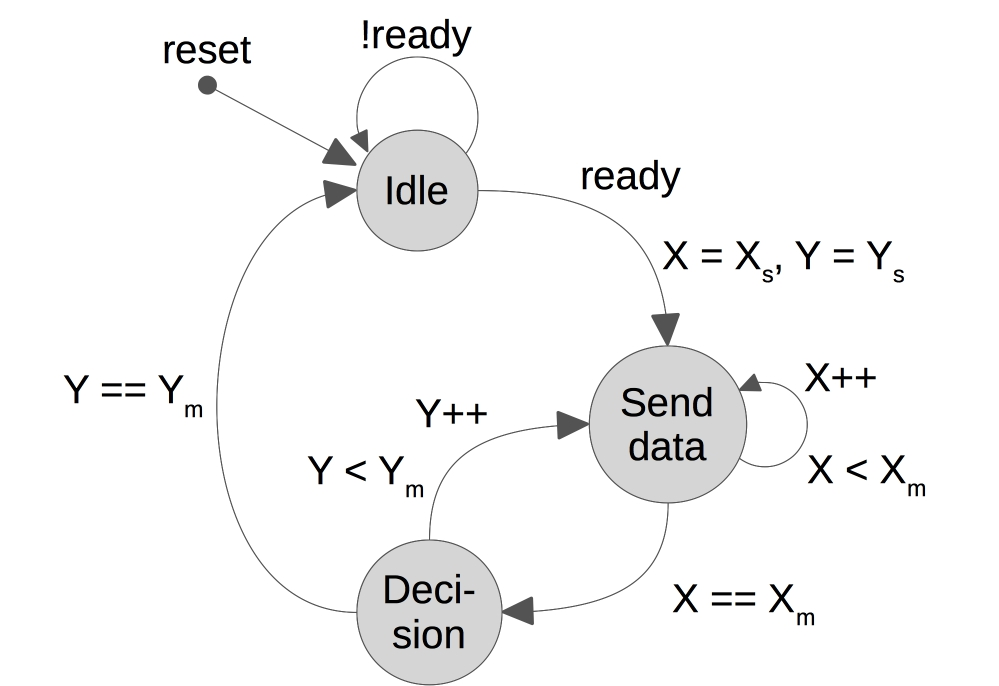
\includegraphics[width=0.5\textwidth]{figures/meanFSMv1.jpg}
  \caption{TEXT GOES HERE}
  \label{fig:LABEL}
\end{figure}

\subsection{Memory}
\begin{figure}
  \centering
  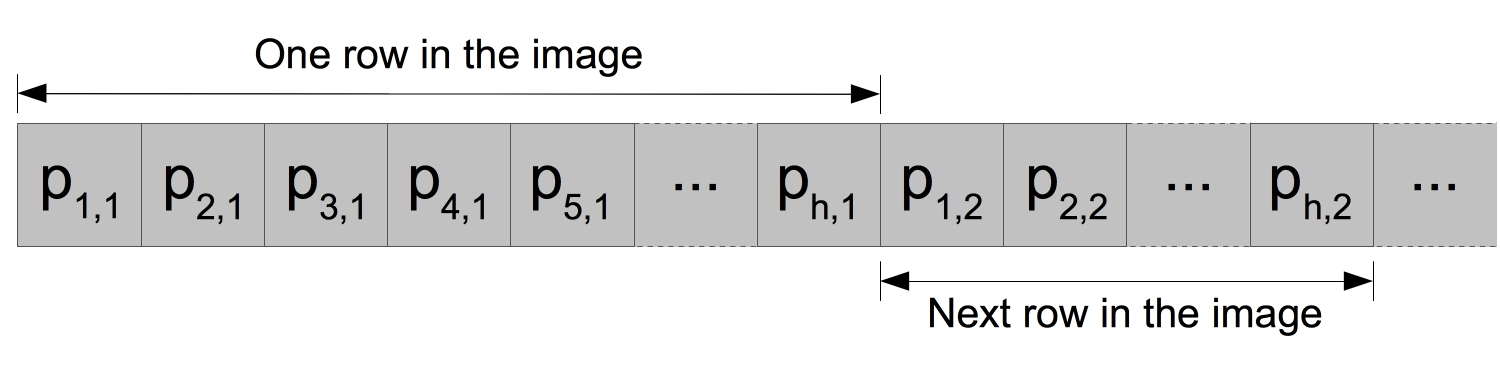
\includegraphics[width=0.5\textwidth]{figures/memdata.jpg}
  \caption{TEXT GOES HERE}
  \label{fig:LABEL}
\end{figure}

memory requirement: \\
$3 \cdot 8$ bits per pixel (rgb image). test image is $741 \times 497$ so for the test image $8.838.648$ bits $\approx$ 9 megabit $\approx$ 1.1 megabyte.

\subsection{VHDL/Simulation}
\todo{skriv om VHDL kode og simulation af filteret}

\subsection{Implementation/Test}
\todo{skriv om implementation på FPGA'en og gerne verificere det virker}



\chapter{Acceptance test}\label{ch:acctest}
\todo{udfør accept test udfra test specifikationen (brug data fra python simulering og giv det til VHDL implementationen)}

\chapter{Conclusion}\label{ch:conclusion}
This chapter concludes on the project. In chapter \vref{ch:introduction} it was specified that the goal of this project was to design and implement a stereo vision algorithm and some questions were to be researched:
\begin{itemize}
  \item What obstacles occur within stereo vision?
  \item Which stereo vision algorithm exist, both being computationally efficient and at the same time providing good vision results?
  \item How can an architecture be designed and optimized for executing a stereo vision algorithm?
\end{itemize}
The findings for each question will be discussed for each question below.
In the end of chapter \vref{ch:introduction} the A$^3$ model were described and in chapter \vref{ch:designmet} the Gajski-Kuhn Y-chart were described. These models were used for structuring the report and project. In the end of this chapter the use of these models will be discussed.

\section*{1 What obstacles occur within stereo vision?}
In chapter \vref{ch:appanalysis} the basics of stereo vision were researched along with some challenges stereo vision brings along with it. With occlusions being a significant subject when discussing stereo vision, occlusions and the different types of occlusions were discussed and different methods to find and fill these occlusions were researched. From this research, it was found that some methods for filling occlusions exists. Four methods were looked at in \cite{huq2013occlusion}. These methods where neighbor's disparity assignment, diffusion in intensity space, segmentation-based least square and weighted least square. The results from that article were used to conclude that a simple occlusion filling method (neighbor's disparity assignment) would be used for this project since the focus is on execution time and the improvement in matching was not high enough for neglect the runtime of the simpler method.\\
Another subject researched in chapter \vref{ch:appanalysis} was the depth precision. HSA Systems requires a high depth precision for future assignments. HSA Systems specified a sensor they wanted to use for the stereo vision system and it was calculated whether the wanted precision where possible to achieve. It was found that the required depth precision was possible to achieve by sacrifice the vertical scene size and using sub-pixel refinement.\\
Other subjects researched where rectification of images and the impact from color spaces. The challenges with rectification were described but for this project, it was not researched further since the test images used are already rectified. For the subject of color spaces the foundings in \cite{chambon2005colour} were used. From this, it was concluded to use grayscale images if the impact on stereo matching quality were not too significant since grayscale images can speed up the runtime but will always have worse stereo matching quality.\\

\section*{2 Which stereo vision algorithm exist, both being computationally efficient and at the same time providing good vision results?}
There exists a lot of stereo vision algorithms but HSA Systems reduced the search to algorithms with a focus on edge preserving algorithms to ensure a good distinction between objects. Two efficient algorithms which preserve the edge were found and these were: Efficient Edge Preserving Stereo Matching and Fast Cost-Volume. In chapter \ref{ch:appanalysis} the algorithms were described and then an algorithm were chosen to be used in this project. For choosing an algorithm both algorithms were simulated in Python and the run-time of each algorithm and the quality of the resulting disparity map were compared. To ensure that the programming skills of the author don't affect the choice of algorithm to use further in the project the theoretical computational complexity of each algorithm were calculated. Both the simulation and the theoretical complexity calculations show that the Efficient Edge Preserving Stereo Matching algorithm is better than the Fast Cost-Volume both when comparing the computational complexity and the quality of the resulting disparity map. Efficient Edge Preserving Stereo Matching was chosen due to the results of the comparison.

\section*{3 How can an architecture be designed and optimized for executing a stereo vision algorithm?}
With an algorithm chosen, the design process towards an architecture could begin. The platform given by HSA Systems was a Zedboard which contains a Zynq Z7020 SoC. The Zynq Z7020 SoC contains both a general purpose processor and an FPGA. This project only focuses on an FPGA implementation hence the GPP part of the platform were not used since this was stated in the project description from HSA Systems. The GPP part was reserved for HSA Systems in case they wanted to use it for other applications in their products.\\

A final FPGA implementation was not achieved in this project but the steps towards an implementation such as scheduling and allocation were described in \ref{ch:archdesign}. It is concluded the architecture design and optimization process for the EEPSM algorithm can follow the general procedure for FPGA design. In the design process, we went through in this project some challenges emerged: the implementation of exponential function and memory usage.\\

The EEPSM algorithm uses exponential function and this function isn't trivial to implement. Different estimates and approximations were looked at: using a power series, using CORDIC and using a lookup table. The power series implementation was unfeasible since it required too many terms and too large constants. Among the CORDIC implementation and the Lookup table implementation, it was found that the lookup table would fit this project the best. This is due to CORDIC being an iterative algorithm and hence will result in higher runtime while lookup table only required an acceptable amount of logic elements since the quantity of numbers used in the exponential function is limited.\\

Another challenge which emerged was a significant memory usage. The algorithm requires saving a lot of copies of the cost images due to the aggregation step. This resulted in the algorithm to require above the available memory on the platform. The algorithm was changed to reduce the memory usage. Two different alterations were considered: Cutting the images into sub-images or down-sampling using image pyramids. The alteration was compared and it were found that the down-sampling altered the resulting disparity map too much to be acceptable while the sub-image alteration didn't affect the algorithm much and hence it were chosen to cut the original images into sub-images.\\

It can be concluded that to implement a stereo vision algorithm using large image sizes then memory usage can be a challenge and have to be optimized. The large images required for a high depth precision also introduces a high disparity range. \\

If the project were to be recreated we would ask to change the project description to include hardware/software co-design implementation instead of only a hardware implementation. This would require learning new theory about hardware/software co-design and use other design models such as the Rugby model \cite{jantsch1999rugby}. The ARM$^\text{\textregistered}$ Processing system contains a NEON engine which is a general-purpose SIMD engine \cite{neon}. The NEON engine works with its own pipeline, register and execution hardware hence it can execute operations parallel with the GPP. The instruction set for the NEON engine include instructions such as MAC by vector, vector minimization, vector multiplication etc. These operations can be multiple parts of the algorithm such as aggregation, SAD, and minimization when finding the disparity value. The inclusion of a GPP can also simplify the memory management. Large images and high disparity ranges require a lot of memory management. The GPP could handle the memory management by controlling pointers to pixels which can be sent to architecture in the FPGA.

\section*{Evaluation of Design Models}
To structure the report the A$^3$ model were used. This model works in three domains and helps limit focus in each domain. i.e. in the first part of report only focus on the application, the second part focus on the algorithm and the last part focus on the architecture.\\
The limiting of focus area can help simplify parts of the design process and limit some of the workload i.e. when researching solutions for occlusion filling the details of implementation in architecture is not considered. This helps to limit the details needed to be considered.\\

To structure the design process of a hardware architecture the Gajski-Kuhn Y-chart were used. This model can help to limit the design process into different domains and abstraction levels. The journey around in the model can be done in different ways i.e. starting at low abstraction levels and moving up in abstraction levels or start at high abstraction levels and moving towards lower levels. It was chosen to follow an FPGA methodology where the design process starts at highest abstraction levels when you have reached a wanted level of abstraction the FPGA software is used to synthesize the design and giving a final implementation. \\

The models helped to structure the project work and in chapter \vref{ch:archdesign} at some occasion examples of information in later domains in the A$^3$ model requires the design process to backtrack into earlier domains to solve challenges. \\

The Gajski-Kuhn Y-chart were feasible for this project since it focuses on a hardware design but if the GPP part of the Zynq SoC were to be used then the Y-chart would be insufficient since the segregation between hardware and software is not naturally modeled in the Y-chart.\\


\printbibliography[heading=bibintoc]
\label{bib:mybiblio}

\appendix
\chapter{Allocation test}
This appendix will explain how the average allocation of logic elements for each functional unit is found.\\
The result is used in table~\vref{tab:utilizationofelements} in chapter \ref{ch:archdesign}. The table is repeated here in table~\vref{tab:apputilizationofelements}

\begin{table}[ht!]
\centering
\begin{tabular}{l | c c c c c }
  \toprule
   &  LUT & LUTRAM & FF & BRAM & DSP48 \\
  \midrule
  Adder & 15 & - & 15 & - & - \\
  Adder/Subtracter  & 16 & - & 15 & - & - \\
  Subtract  & 15 & - & 15 & - & - \\
  Multiplier - LUT  & 352 & - & 36 & - & - \\
  Multiplier - DSP48 & - & - & - & - & 1 \\
  Divider & 680 & 1 & 150 & 0.5 & 8 \\
  \bottomrule
\end{tabular}
\caption{Number of logic elements used in average for each FU}
\label{tab:apputilizationofelements}
\end{table}

\section{General procedure}
This section will describe the general procedure to find the utilization of logic elements for the specified FUs. 

First a new project is created in Xilinx Vivado 2016.2. All the settings are set to standard except for the target which is set to ZedBoard Zynq Evaluation and Development Kit. Then a block design is created and a single IP of the wanted type is added. Then for each input and output a port is generated and connected to the inputs and outputs. Using TCL commands the IP block is copied 99 times and for each copy a new output port is generated and connected to the copy. The inputs are all connected the original corresponding ports except for the divider FU where each copy will have its own input ports. When everything have been connected then Vivado is set to generate top-level HDL wrapper for the block design. Run a synthesis and after completion check the utilization table under the project summary. These values should be divided by 100 and inserted into table~\vref{tab:apputilizationofelements}

The following sections will describe the specific settings for each FUs. 

\section{Adder}
This FU uses the Xilinx Adder/Subtracter v12.0 LogiCORE IP. The IP is set to implement using \textit{Fabric}. The inputs are set to a width of 15 bits, mode is set to \textit{add} and the output is set to 15 bits and latency is set to 1. All control signals are disabled.

\section{Subtract}
This FU uses the Xilinx Adder/Subtracter v12.0 LogiCORE IP. The IP is set to implement using \textit{Fabric}. The inputs are set to a width of 15 bits, mode is set to \textit{subtract} and the output is set to 15 bits and latency is set to 1. All control signals are disabled.

\section{Adder/Subtract}
This FU uses the Xilinx Adder/Subtracter v12.0 LogiCORE IP. The IP is set to implement using \textit{Fabric}. The inputs are set to a width of 15 bits, mode is set to \textit{add subtract} and the output is set to 15 bits and latency is set to 1. All control signals beside the ADD signal are disabled.

\section{Multiplier - LUT}
This FU uses the Xilinx Multiplier v12.0 LogiCORE IP. The IP is set to construct the multiplier using \textit{LUTs} and is set to optimize for speed. The inputs are set to a width of 18 bits and the output is set to 36 bits and pipeline stages is set to 1. All control signals are disabled.

\section{Multiplier - DSP48}
This FU uses the Xilinx Multiplier v12.0 LogiCORE IP. The IP is set to construct the multiplier using \textit{Mults} and is set to optimize for speed. The inputs are set to a width of 18 bits and the output is set to 36 bits and pipeline stages is set to 1. All control signals are disabled.

\section{Divider}
This FU uses the Xilinx Divider Generator v5.1 LogiCORE IP. The algorithm type is set to \textit{High Radix}. The inputs are set to a width of 16 bits and the output fractional width is set to 16 bits and latency is set to 4. All control signals are disabled.
\chapter{Extra Figures}
\color{gray}
\section*{noter til mig selv}
% ---------------------- udkommentere senere --------****
This chapter will contain extra which might fill to much in the report. Looking at you precedence graphs.
Maybe make it as fold out image as we did with large diagrams in earlier reports.
\color{black} 
\chapter{Middlebury data set}\label{app:middlebury}
This appendix contains a brief description over the data sets from Middlebury. The computer vision department at Middlebury College have a large library of stereo pair with ground truth\cite{middlebury2016}. These data sets are used all around the world for evaluating stereo vision algorithms. This thesis uses a subset of these stereo pairs. \\
These are: Tsukuba, Cones, Teddy and Motorcycle. The three first data sets are used due to great knowledge of them from HSA systems. The last set, Motorcycle, is used due to it having the ground truth as an .pfm file. With a .pfm file then comparing is easier since the ground truth for other sets have scaling hence direct comparison is not possible. The four data sets are presented below.\\

\begin{figure}[ht]
  \centering
  \begin{subfigure}[t]{0.3\textwidth}
    \centering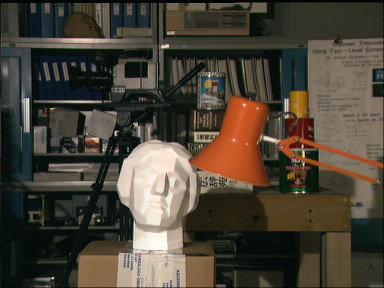
\includegraphics[width=0.9\textwidth]{figures/tsul.jpg}
    \caption{Left image \label{fig:aptsu_l}}
  \end{subfigure}\hspace{0.5cm}
  \begin{subfigure}[t]{0.3\textwidth}
    \centering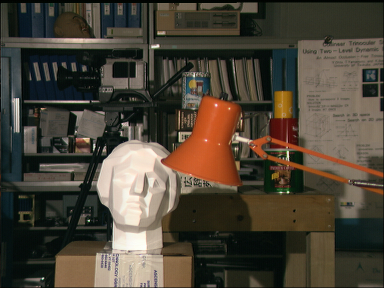
\includegraphics[width=0.9\textwidth]{figures/tsur}
    \caption{Right image\label{fig:aptsu_r}}
  \end{subfigure}\hspace{0.5cm}
  \begin{subfigure}[t]{0.3\textwidth}
    \centering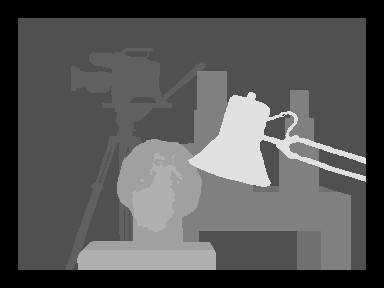
\includegraphics[width=0.9\textwidth]{figures/tsu_gt}
    \caption{Ground Truth\label{fig:aptsu_gt}}
  \end{subfigure}
  \caption{Tsukuba - $384\times288$ \cite{Scharstein2002}\label{fig:aptsu}}
\end{figure}

\begin{figure}[ht]
  \centering
  \begin{subfigure}[t]{0.3\textwidth}
    \centering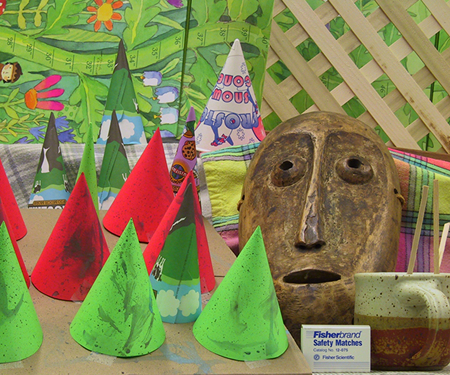
\includegraphics[width=0.9\textwidth]{figures/conl.jpg}
    \caption{Left image \label{fig:apcon_l}}
  \end{subfigure}\hspace{0.5cm}
  \begin{subfigure}[t]{0.3\textwidth}
    \centering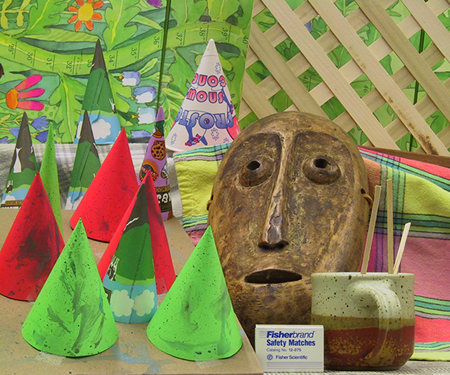
\includegraphics[width=0.9\textwidth]{figures/conr}
    \caption{Right image\label{fig:apcon_r}}
  \end{subfigure}\hspace{0.5cm}
  \begin{subfigure}[t]{0.3\textwidth}
    \centering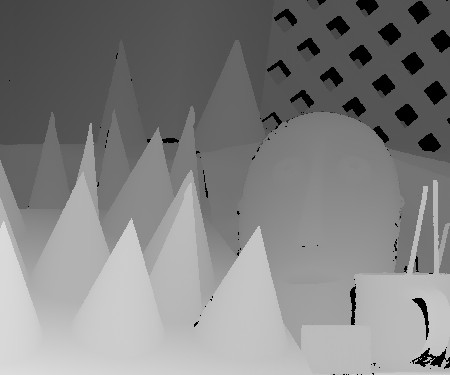
\includegraphics[width=0.9\textwidth]{figures/con_gt}
    \caption{Ground Truth\label{fig:apcon_gt}}
  \end{subfigure}
  \caption{Cones - $450\times375$ \cite{Scharstein2003}\label{fig:apcon}}
\end{figure}

\begin{figure}[ht]
  \centering
  \begin{subfigure}[t]{0.3\textwidth}
    \centering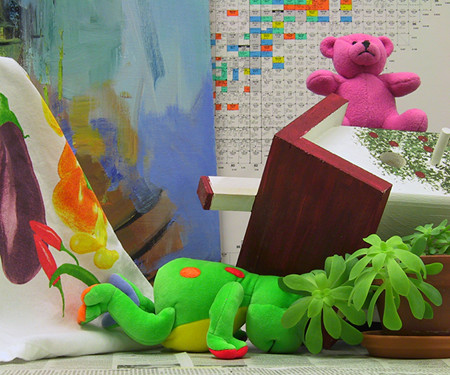
\includegraphics[width=0.9\textwidth]{figures/tedl.jpg}
    \caption{Left image \label{fig:apted_l}}
  \end{subfigure}\hspace{0.5cm}
  \begin{subfigure}[t]{0.3\textwidth}
    \centering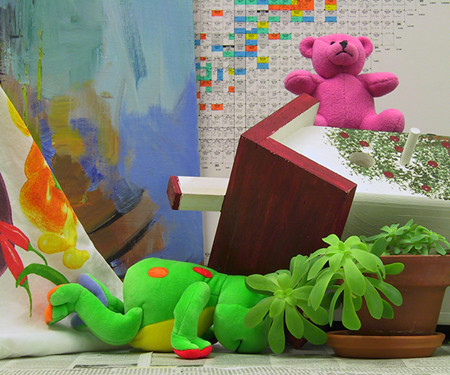
\includegraphics[width=0.9\textwidth]{figures/tedr}
    \caption{Right image\label{fig:apted_r}}
  \end{subfigure}\hspace{0.5cm}
  \begin{subfigure}[t]{0.3\textwidth}
    \centering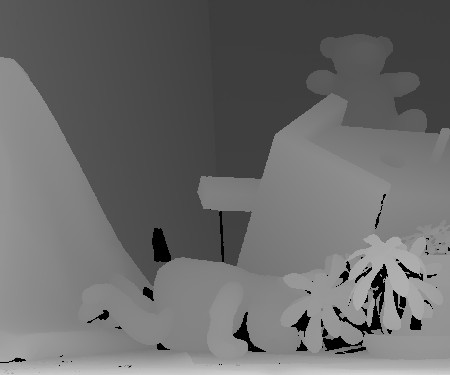
\includegraphics[width=0.9\textwidth]{figures/ted_gt}
    \caption{Ground Truth\label{fig:apted_gt}}
  \end{subfigure}
  \caption{Teddy - $450\times375$ \cite{Scharstein2003}\label{fig:apted}}
\end{figure}

\begin{figure}[ht]
  \centering
  \begin{subfigure}[t]{0.3\textwidth}
    \centering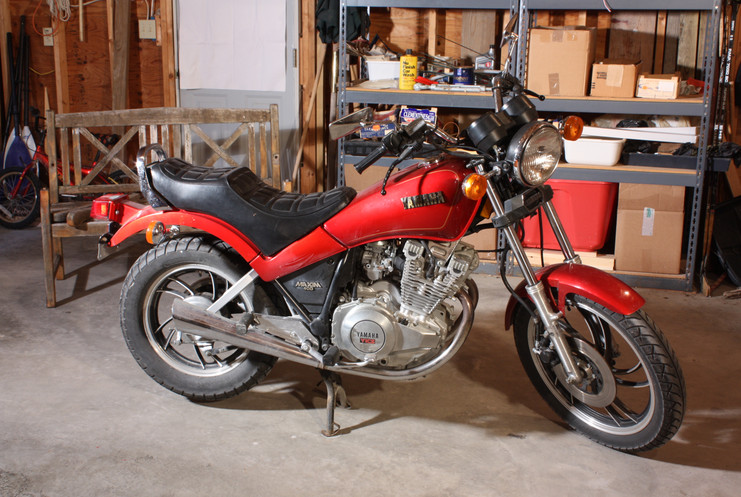
\includegraphics[width=0.9\textwidth]{figures/motl.jpg}
    \caption{Left image \label{fig:apmot_l}}
  \end{subfigure}\hspace{0.5cm}
  \begin{subfigure}[t]{0.3\textwidth}
    \centering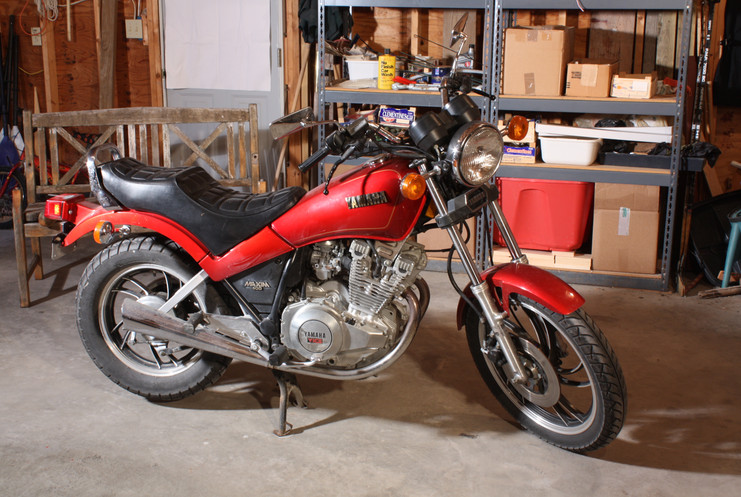
\includegraphics[width=0.9\textwidth]{figures/motr}
    \caption{Right image\label{fig:apmot_r}}
  \end{subfigure}\hspace{0.5cm}
  \begin{subfigure}[t]{0.3\textwidth}
    \centering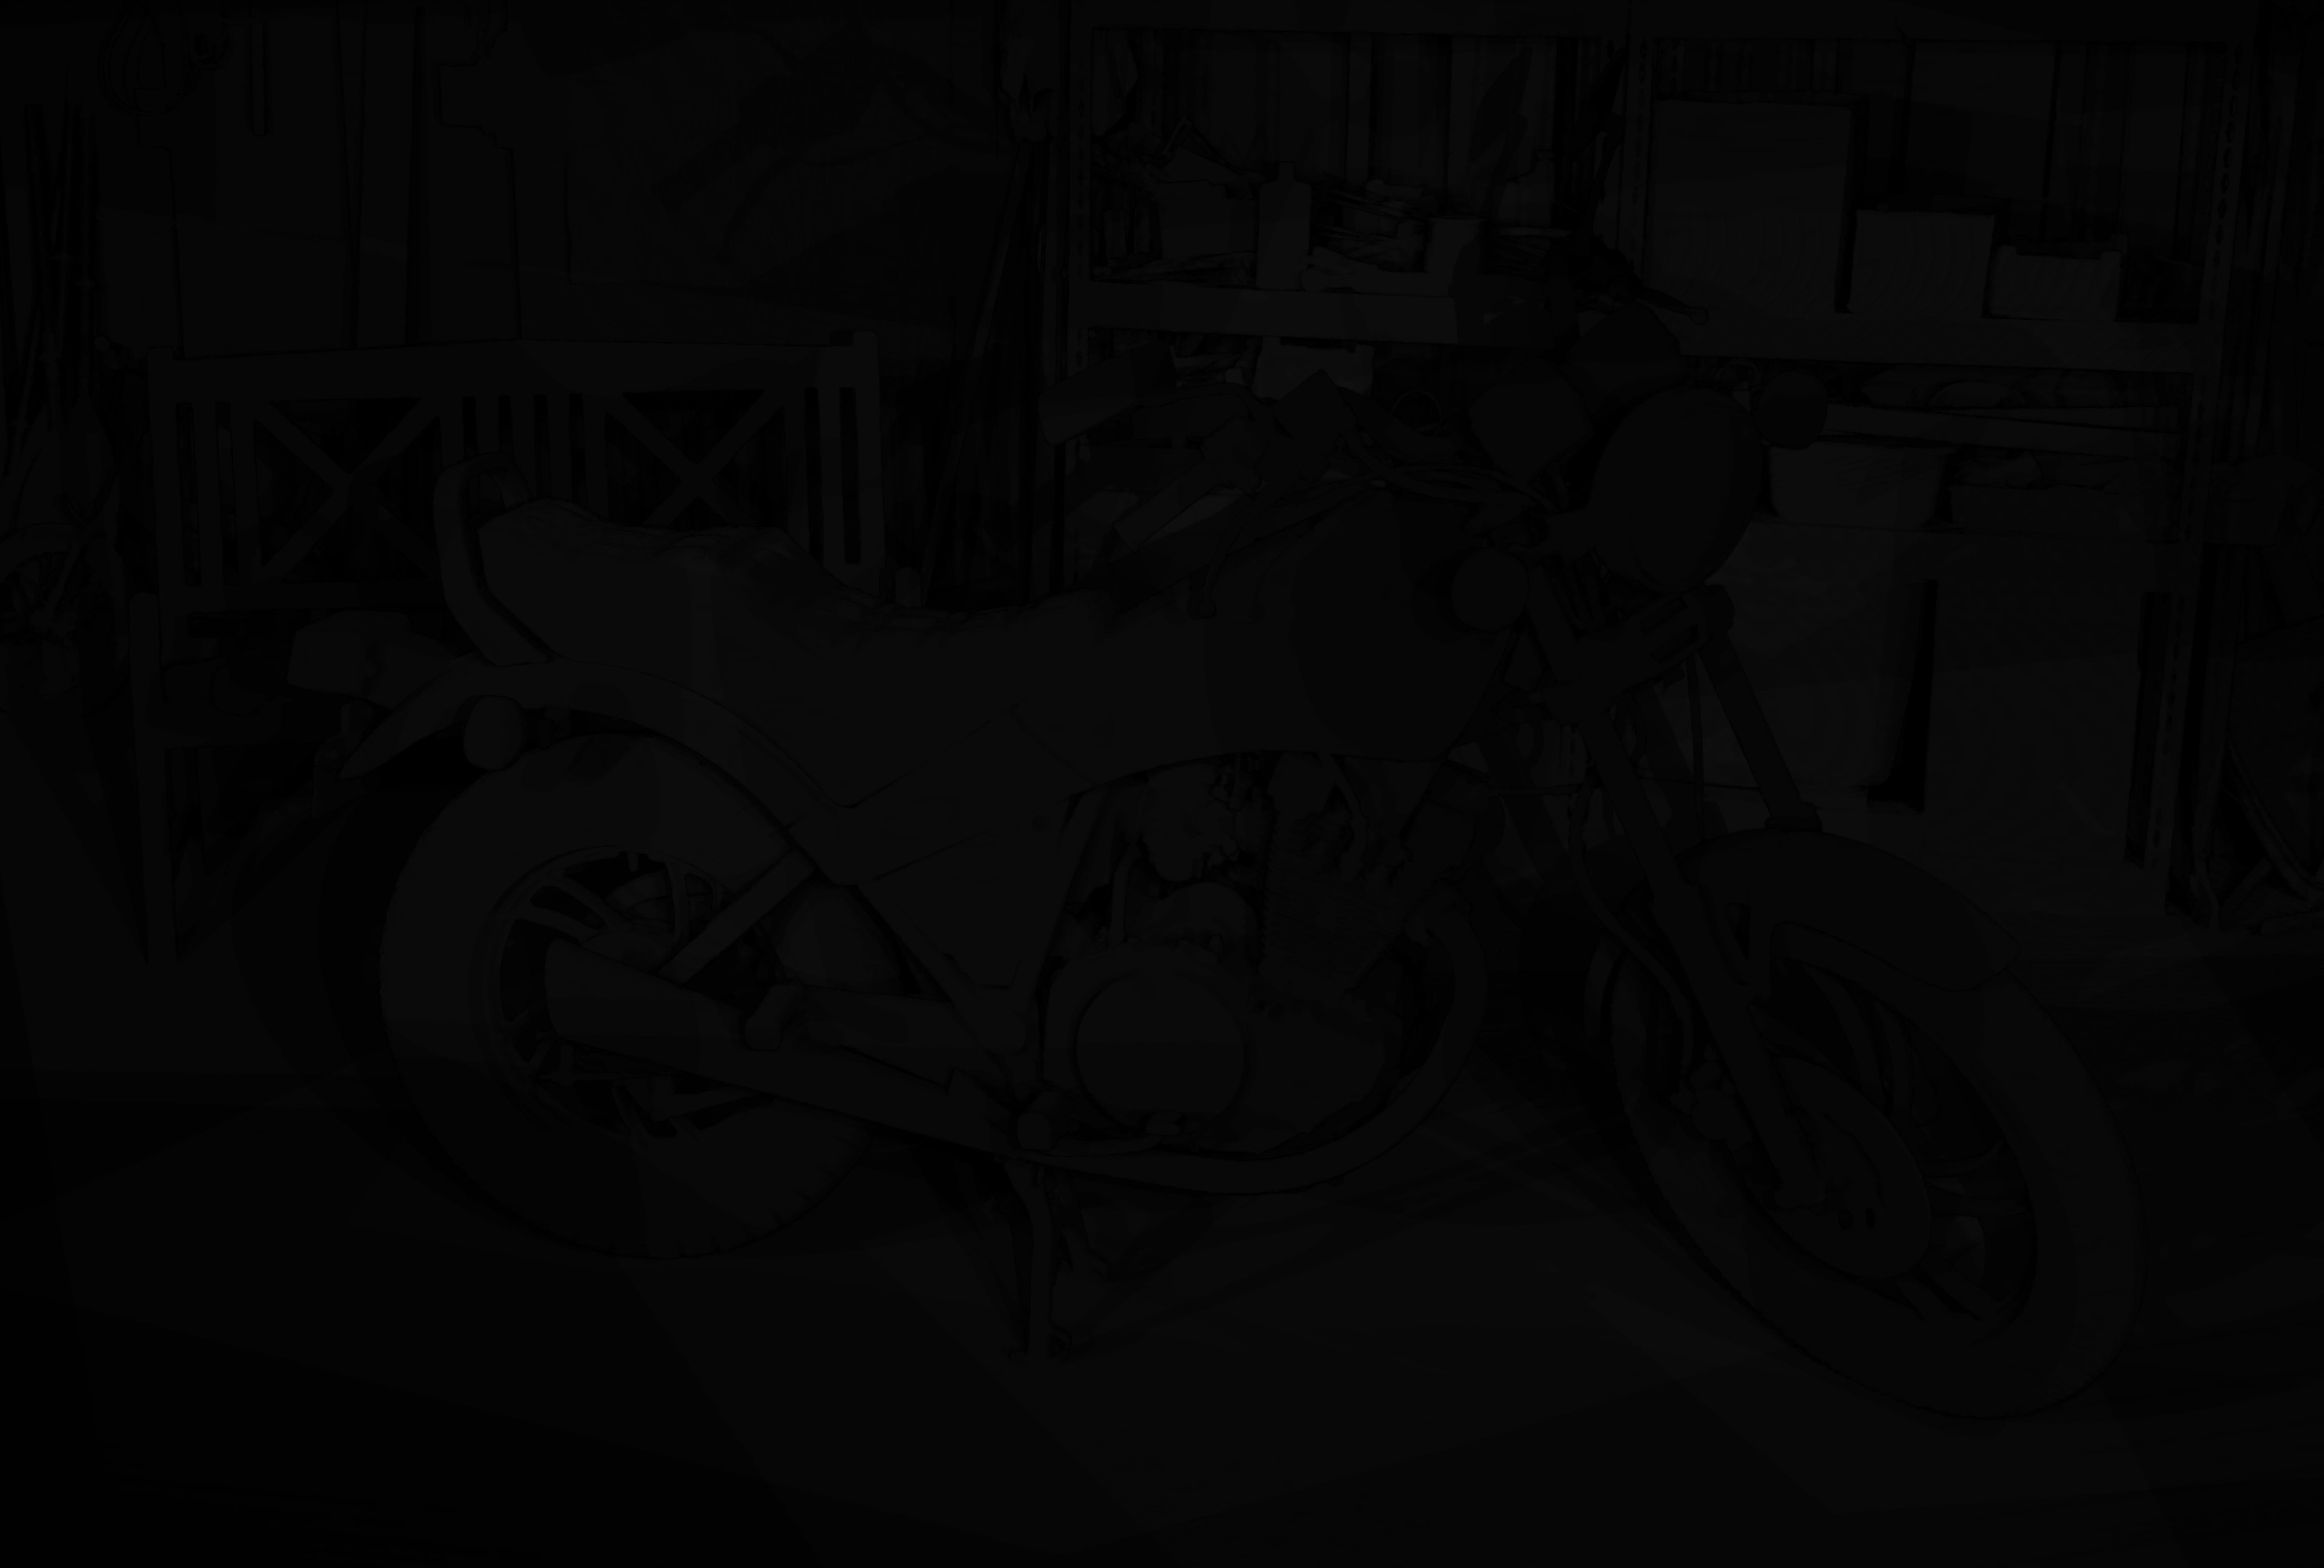
\includegraphics[width=0.9\textwidth]{figures/mot_GT}
    \caption{Ground Truth\label{fig:apmot_gt}}
  \end{subfigure}
  \caption{Motorcycle - $741\times497$ \cite{Scharstein2014}\label{fig:apmot}}
\end{figure}
\end{document}
